% ----------------------- TODO ---------------------------
% Diese Daten müssen pro Blatt angepasst werden:
\newcommand{\NUMBER}{1}
\newcommand{\EXERCISES}{5}
% Diese Daten müssen einmalig pro Vorlesung angepasst werden:
\newcommand{\COURSE}{HPC Lab - Assignment 2}

\newcommand{\STUDENTA}{Zirong Cai}
\newcommand{\STUDENTB}{Phuong Nguyen}
\title{\vspace{-2em} Assignment 2 - OpenMP \vspace{-0.5em}}
\author{ \STUDENTA, \STUDENTB}
\date{\today {\vspace{-1cm}}}

% ----------------------- TODO ---------------------------

\documentclass[article]{scrartcl}

\usepackage[utf8]{inputenc}
\usepackage[ngerman]{babel}
\usepackage{amsmath}
\usepackage{amssymb}
\usepackage{fancyhdr}
\usepackage{color}
\usepackage{graphicx}
\usepackage{lastpage}
\usepackage{listings}
\usepackage{tikz}
\usepackage{pdflscape}
\usepackage{subfigure}
\usepackage{float}
\usepackage{polynom}
\usepackage{hyperref}
\usepackage{tabularx}
\usepackage{forloop}
\usepackage{geometry}
\usepackage{listings}
\usepackage{caption}
\usepackage{fancybox}
\usepackage{tikz}
\usepackage{algpseudocode,algorithm,algorithmicx}
%\usepackage{biblatex}
\usepackage{cite}

\setkomafont{title}{\normalsize}
\setkomafont{author}{\small}
\setkomafont{date}{\small}
\setkomafont{section}{\normalfont \normalsize \textbf}
\setkomafont{subsection}{\normalfont}
\renewcommand*{\thesubsection}{\alph{subsection}}

\setkomafont{subsubsection}{\normalfont\itshape}

\lstset { %
    language=C++,
    backgroundcolor=\color{black!5}, % set backgroundcolor
    basicstyle=\footnotesize,% basic font setting
}
%\captionsetup[lstlisting]{ format=listings, labelfont=white, textfont=white}

%Definiere Let-Command für algorithmen
%\newcommand*\Let[2]{\State #1 $\gets$ #2}

%\input kvmacros

%Größe der Ränder setzen
\geometry{a4paper,left=3cm, right=3cm, top=3cm, bottom=3cm}

%Kopf- und Fußzeile
\pagestyle {fancy}
\fancyhead[L]{\STUDENTA, \STUDENTB}
\fancyhead[R]{\COURSE}

\fancyfoot[L]{}
\fancyfoot[R]{Page \thepage /\pageref*{LastPage}}

\begin{document}


\maketitle
\thispagestyle{fancy}

%% Listing code
%\begin{lstlisting}[frame=single]
%
%\end{lstlisting}
%------------------------------
% Inserting figures
%\begin{figure}[htpb]
%    \centering
%    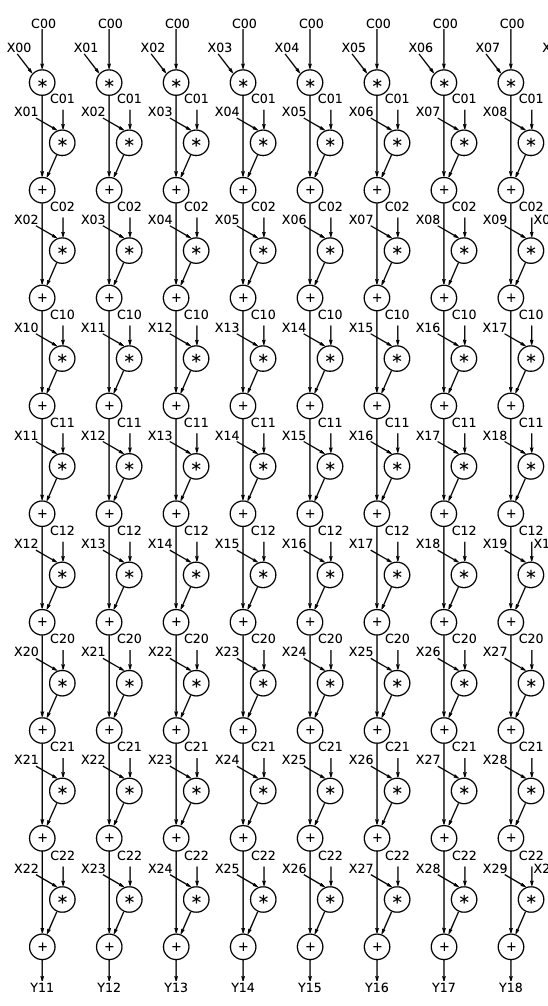
\includegraphics[width=\textwidth,height=6cm,keepaspectratio=true]{../figs/2D_strategy.png}
%    \caption{}
%    \label{}
%\end{figure}
%------------------------------
%% Simple table
%\begin{center}
%\begin{tabular}{ |c|c| } 
% \hline
%
% \hline
%\end{tabular}
%\end{center}

\section{Shared memory Pi-calculation (2P)}
\subsection{Theory}
\begin{figure}[h]
  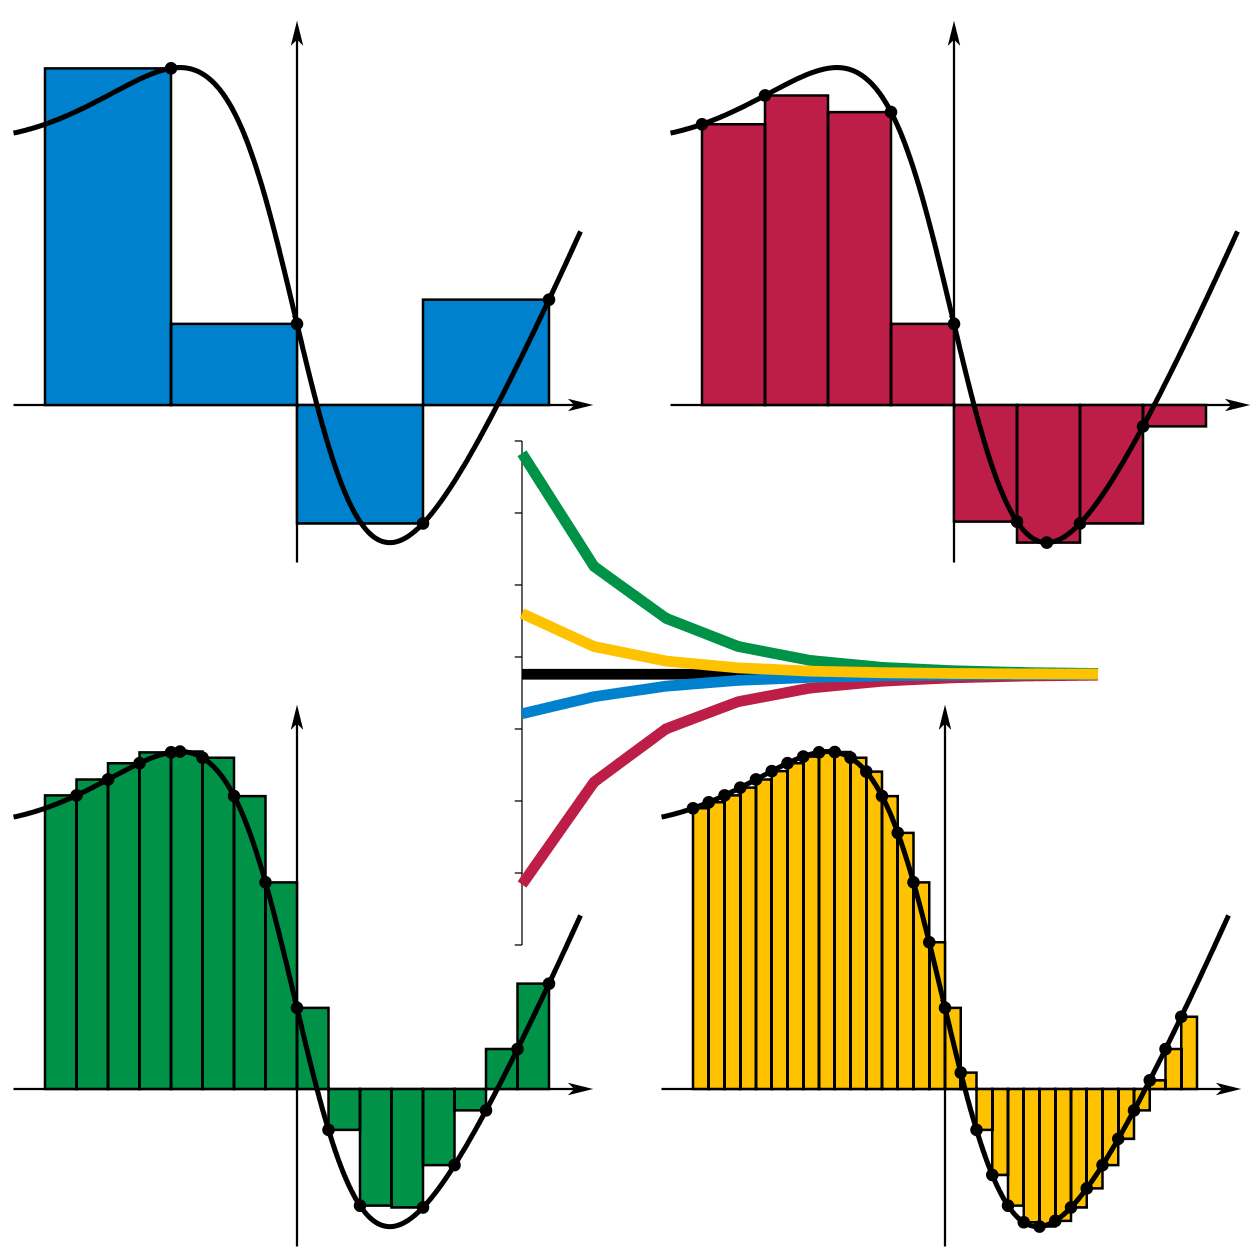
\includegraphics{../figs/Riemann_sum_convergence.png}
  \centering
  \caption{Riemann Sum\cite{riemannsum}}
  \label{fig:riemann}
\end{figure}
In mathematics, a Riemann sum is a certain kind of approximation of an integral by a finite sum.
As shown in Figure \ref{fig:riemann}, the Riemann sum is defined as:
$$
S = \sum_{i=1}^{n}f(x^{*})\Delta x_i
$$ 
where $f(x)$ is a function defined in [a,b], and 
$$P=\{[x_0,x_1],[x_1,x_2]... [x_{n-1},x_n]\}, a = x_0 < x_1 < ...<x_{n-1}<x_n=b$$
is a partion of [a,b], $\Delta x_i = x_i - x_{i-1}$ is the width of every rectangle.
As $\Delta x_i$ approaches to zero, the integration of function $f(x)$ approaches to the accurate number.
\\
There are many different variates of choosing $x^{*}$, one can choose the left boundary of the partition which 
result in Left Riemann Sum, or choose the right boundary leads to Right Riemann Sum. Here in this program, we 
choose the midpoint as our $x^*$.\\
To calculate the integration:
$$
\int_{0}^1\frac{1}{1+x^2}dx
$$
we first split interval [0,1] into n equal sized subinterval with width $\Delta x$ equals to $\frac{1}{n}$.
So in our case, The Partition P is defined as:
$$P=\{[0,\frac{1}{n}],[\frac{1}{n},\frac{2}{n}]... [\frac{n-1}{n},1]\}$$

\subsection{Code}
Serial version:
\begin{lstlisting}[frame=single]
  double pi_integrate_serial(double start, double end, int precision)
  {
      double length = (end - start ) / precision;
      double x = length/2.0;
      double sum = 0;
      for (size_t i = 0; i < precision; i++)
      {
          double tmp = pi_func(x + i*length);
          sum += tmp;
      }
      return 4 * sum * length; 
  }
\end{lstlisting}
Critical version:  
\begin{lstlisting}[frame=single]
  double pi_integrate_critical(double start, double end, int precision)
  {
      double length = (end - start ) / precision;
      double x = length/2.0;
      double sum = 0;
      #pragma omp parallel for shared(x, length, sum), schedule(static)
      for (size_t i = 0; i < precision; i++)
      {
          double tmp = pi_func(x + i*length);
          #pragma omp critical
          sum += tmp;
      }
      return 4 * sum * length; 
  }
\end{lstlisting}
Reduction Version:
\begin{lstlisting}[frame=single]
  double pi_integrate_reduction(double start, double end, int precision)
  {
      double length = (end - start ) / precision;
      double x = length/2.0;
      double sum = 0;
      #pragma omp parallel for shared(x, length), schedule(static), \
                               reduction(+: sum)
      for (size_t i = 0; i < precision; i++)
      {
          double tmp = pi_func(x + i*length);
          sum += tmp;
      }
      return 4 * sum * length;
  }
\end{lstlisting}
\subsection{Evaluation}
\begin{figure}[ht]
  \begin{subfigure}
    \centering
    % include first image
    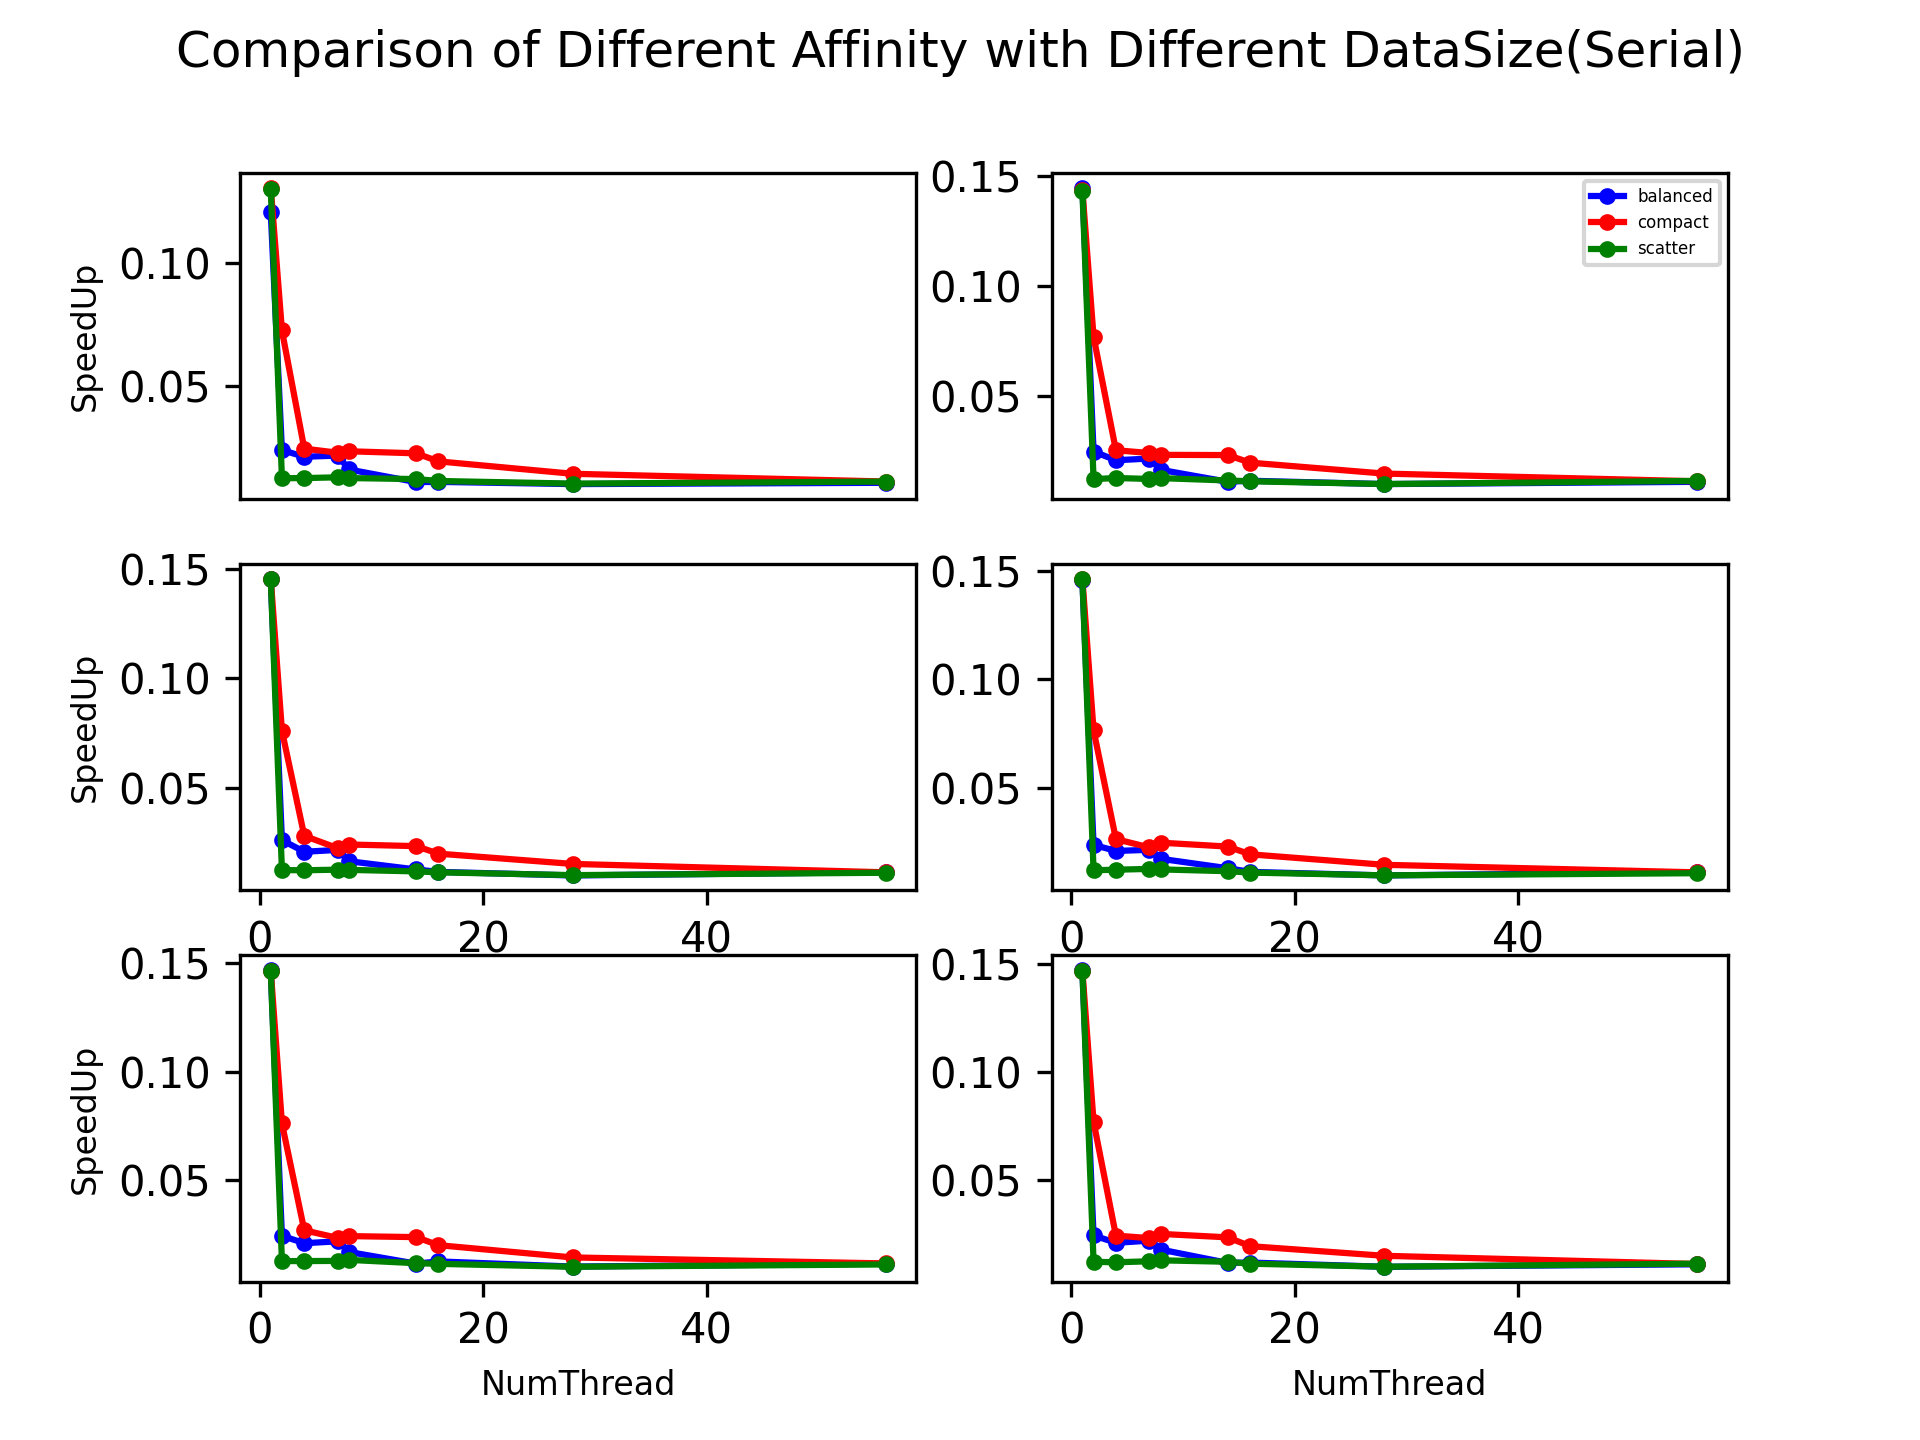
\includegraphics[width=.5\linewidth]{../figs/Compare_Aff_AllinOne_serial.png}  
    \label{fig:critical}
  \end{subfigure}
  \begin{subfigure}
    \centering
    % include second image
    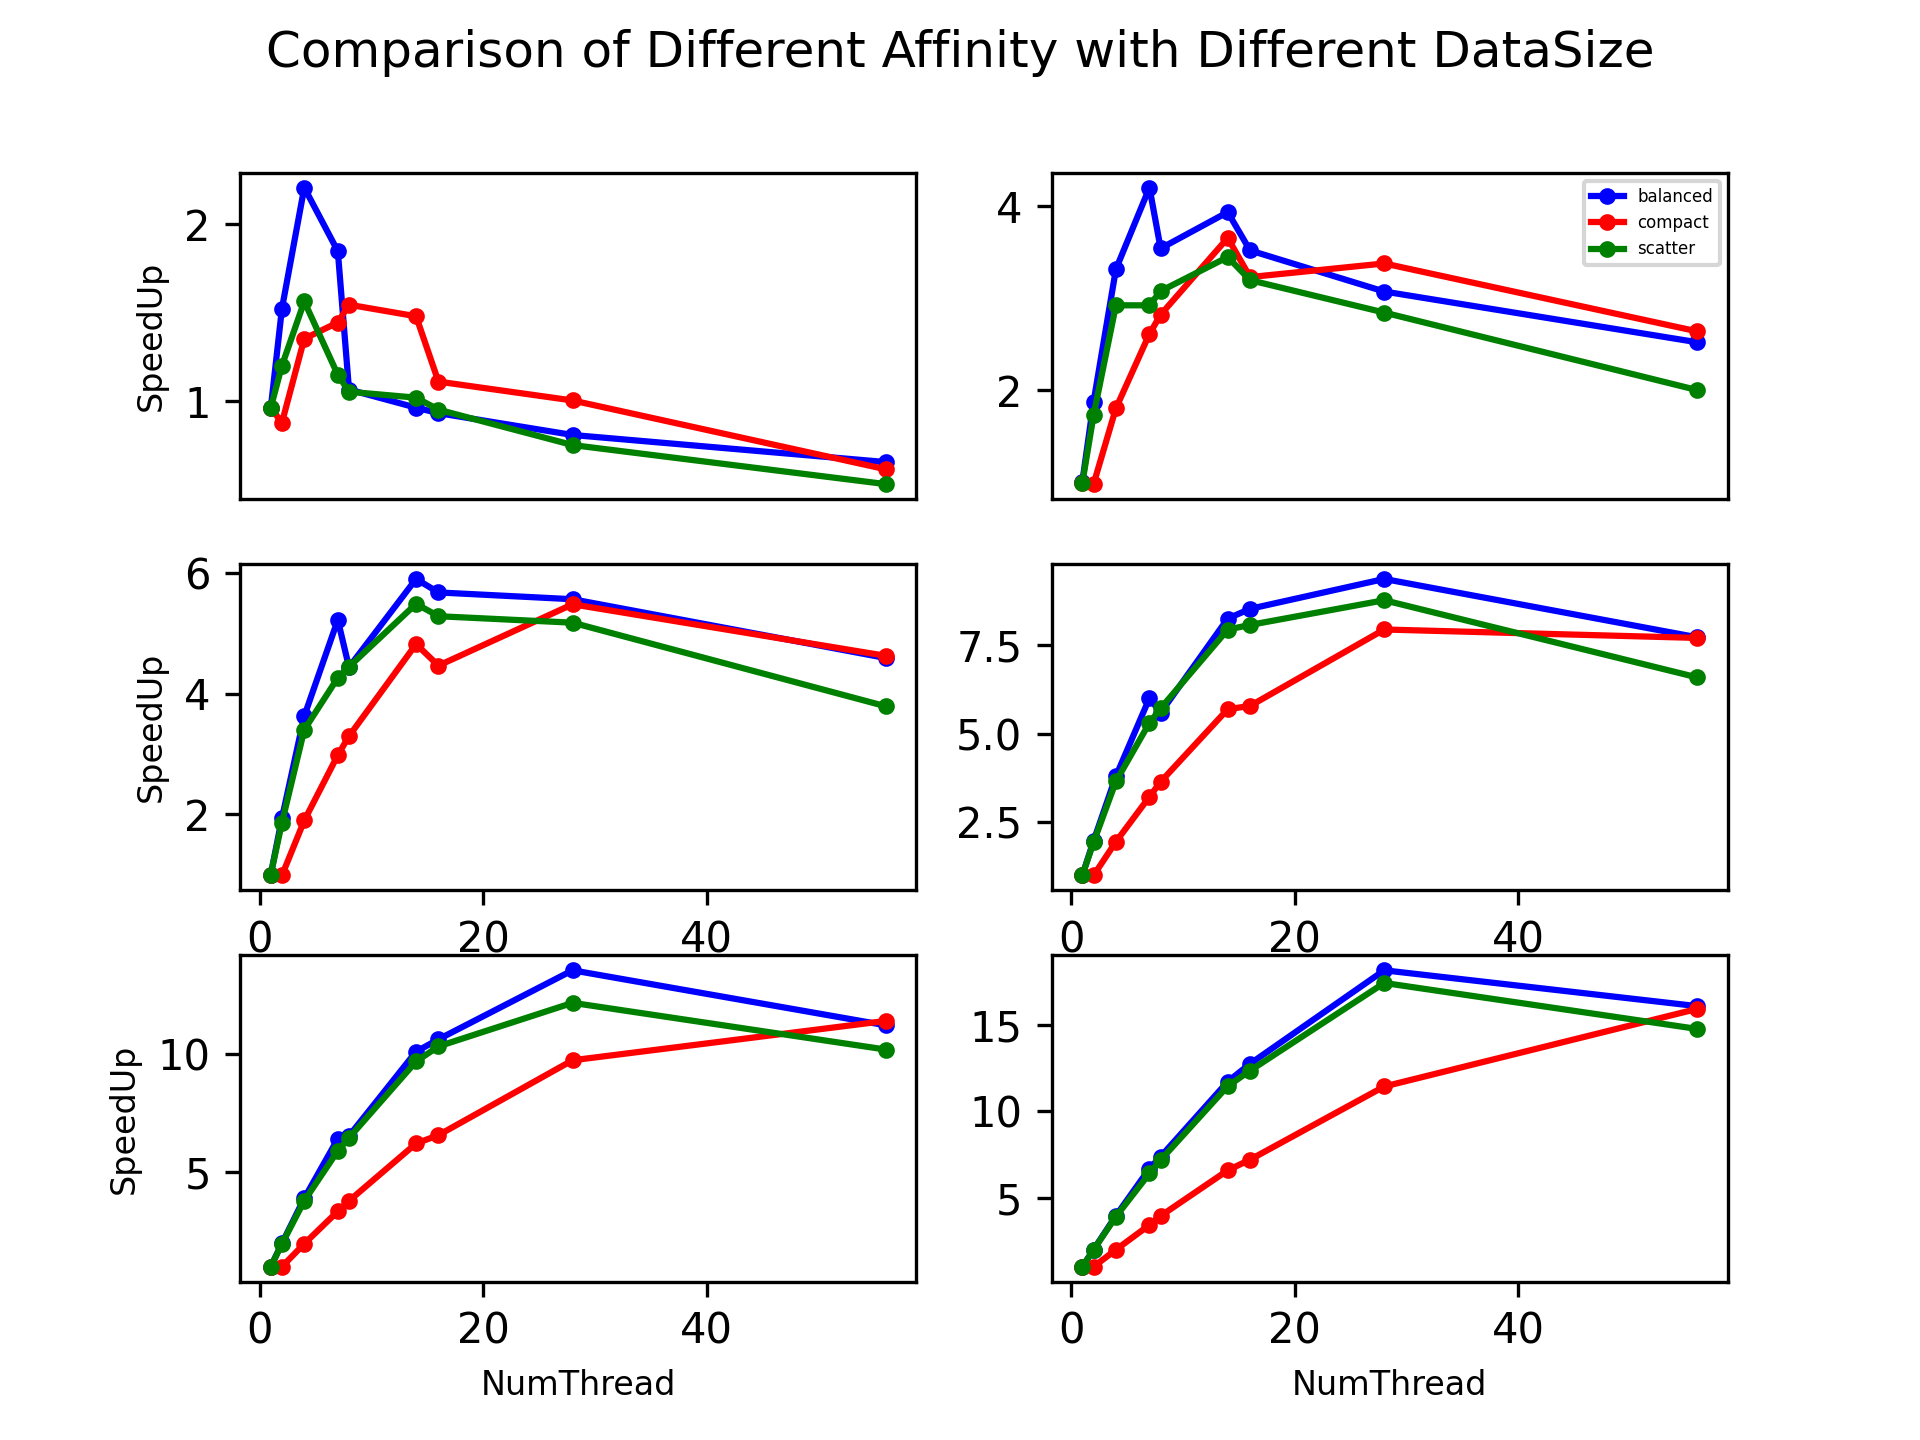
\includegraphics[width=.5\linewidth]{../figs/Compare_Aff_AllinOne.png}  
    \label{fig:reduction}
  \end{subfigure}
  \caption{Strong Scaling with Different Affinity and Different DataSize(Critical and Reduction), Data size from top to down
  are 1000,2000,4000,8000,16000,28000,56000}
  \label{fig:compareAff}
  \end{figure}
  To see how our program performs in different affinity mode(balanced, compact, scatter),
  We tested the program with different data size and thread number. As shown in \ref{fig:compareAff}, 
  the critical version runs much slower than the serial version, because all threads need to write to 
  the sum variable which is critical, that means, the critical version act like the serial version but with much more additional
  overhead caused by thread create and thread communication. \textbf{We thus conclude that reduction version scales better regarding to strong scaling.}\\
  In Figure \ref{fig:compareAff}(right), we can see that when data size is small, compact mode performs better when higher thread number is set,
  but as the data size grows, balanced mode becomes more powerful. This Figure also shows the strong scaling of our program.
  For the last three plots(data size = 16000,28000,56000), the speedup reaches the highest value when thread number equals to 28,
  namely, one thread per core. Since our function is just doing some basic mathmatic calculation, hyperthreading does not help to improve the performance here.
  It's also intersting to point out that in the first three plots(data size = 1000,2000,4000), there's a performance decrease between NumThread = 7, 8 and NumThread = 14, 16,
  because CM2 is a NUMA system and each include 7 cores, so the extra thread may need to process the data that far away from it and thus cause more overheads.

  \begin{figure}[ht]
    \begin{subfigure}
      \centering
      % include first image
      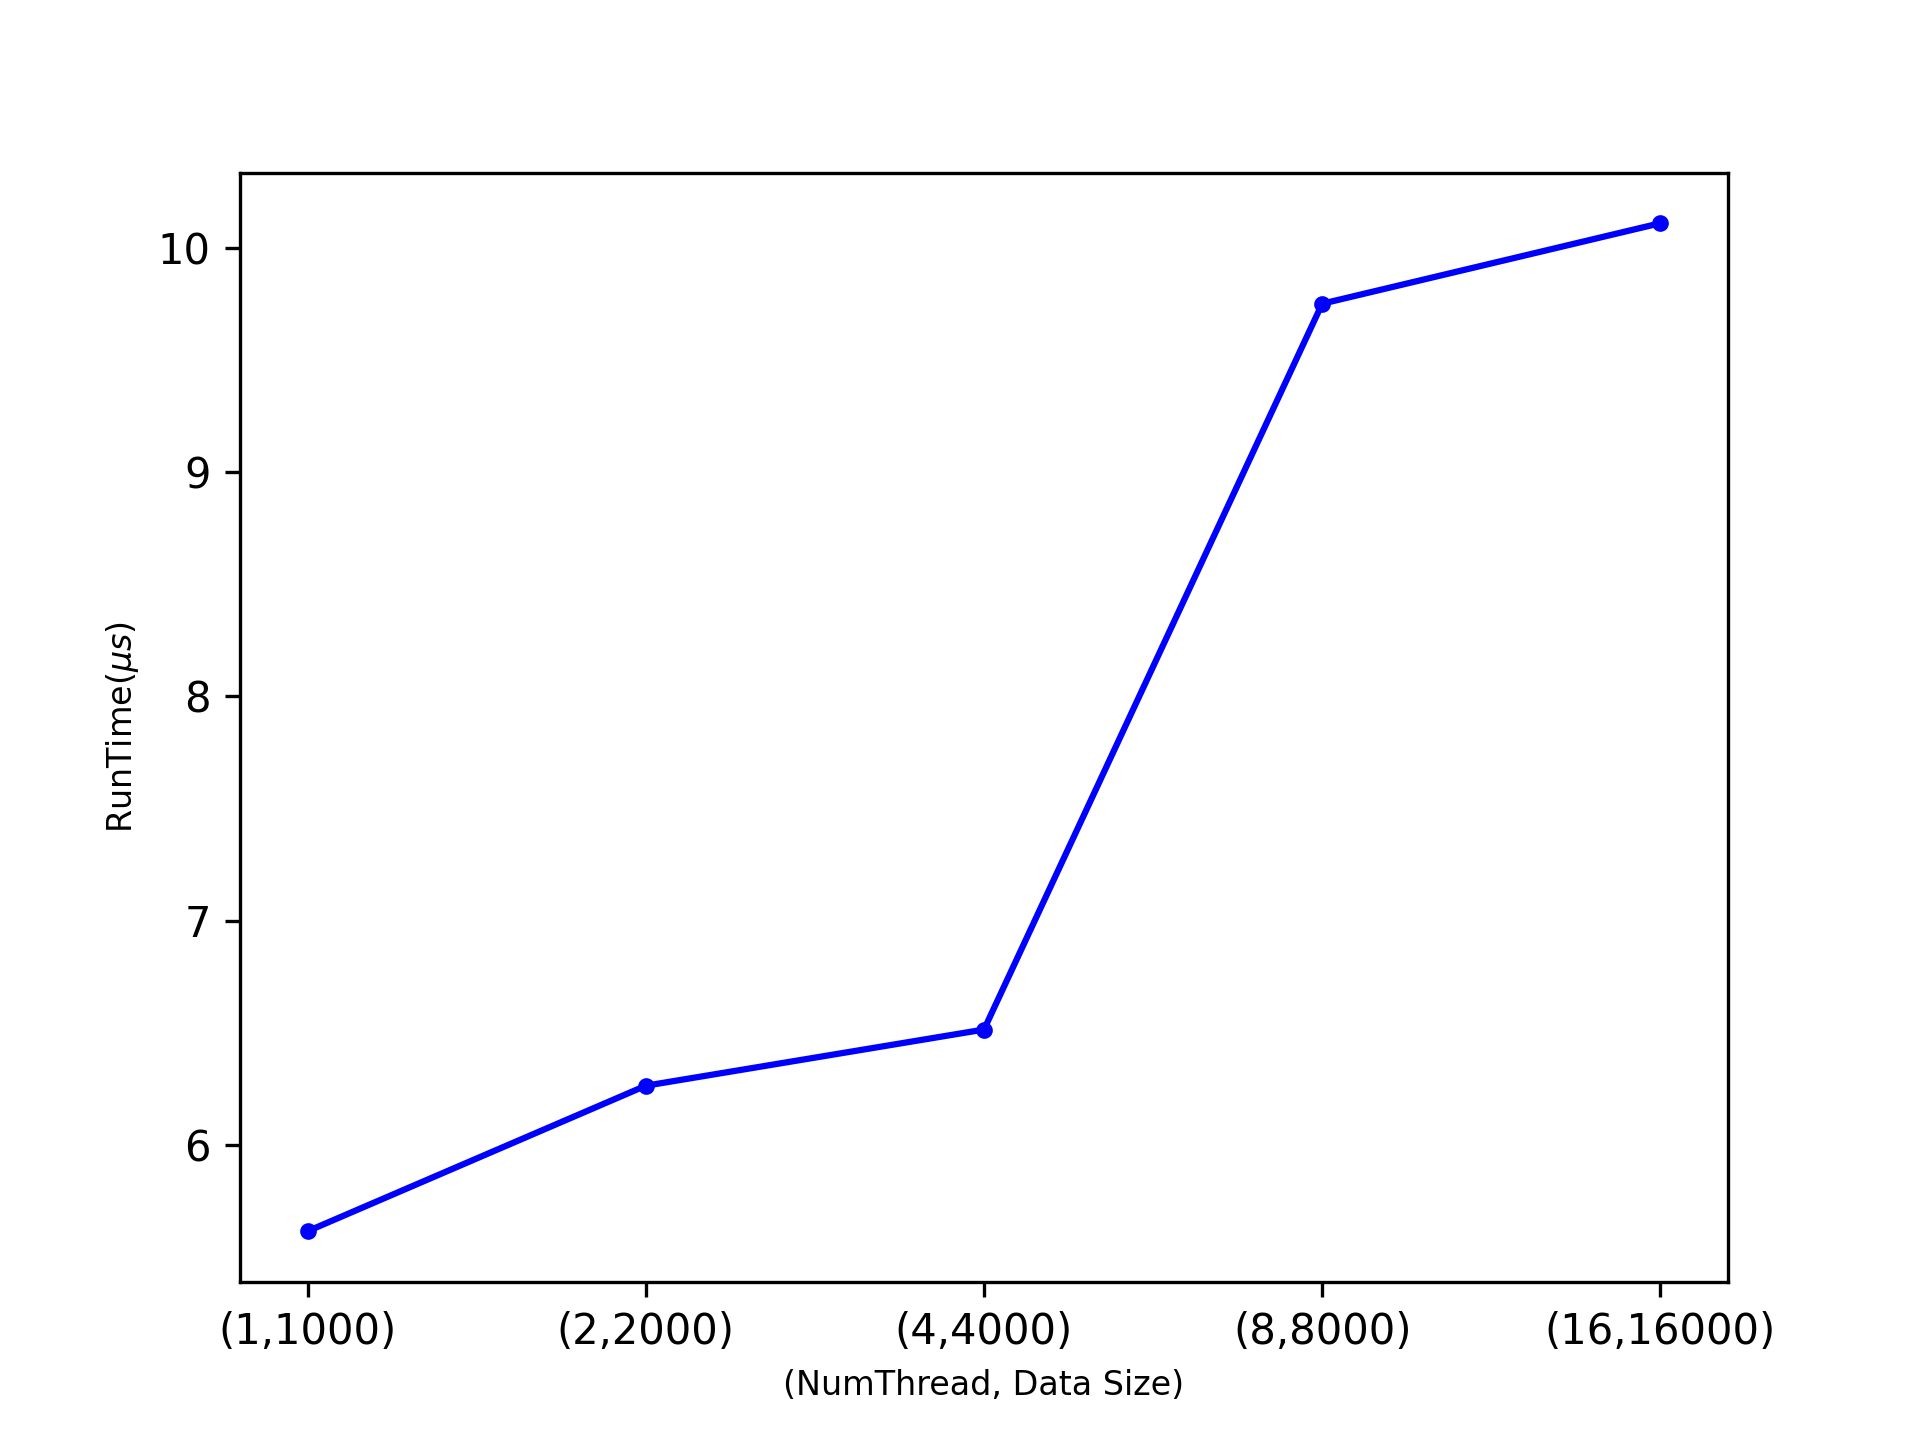
\includegraphics[width=.5\linewidth]{../figs/WeakScaling1_AllinOne.png}  
      \label{fig:WeakScaling1}
    \end{subfigure}
    \begin{subfigure}
      \centering
      % include second image
      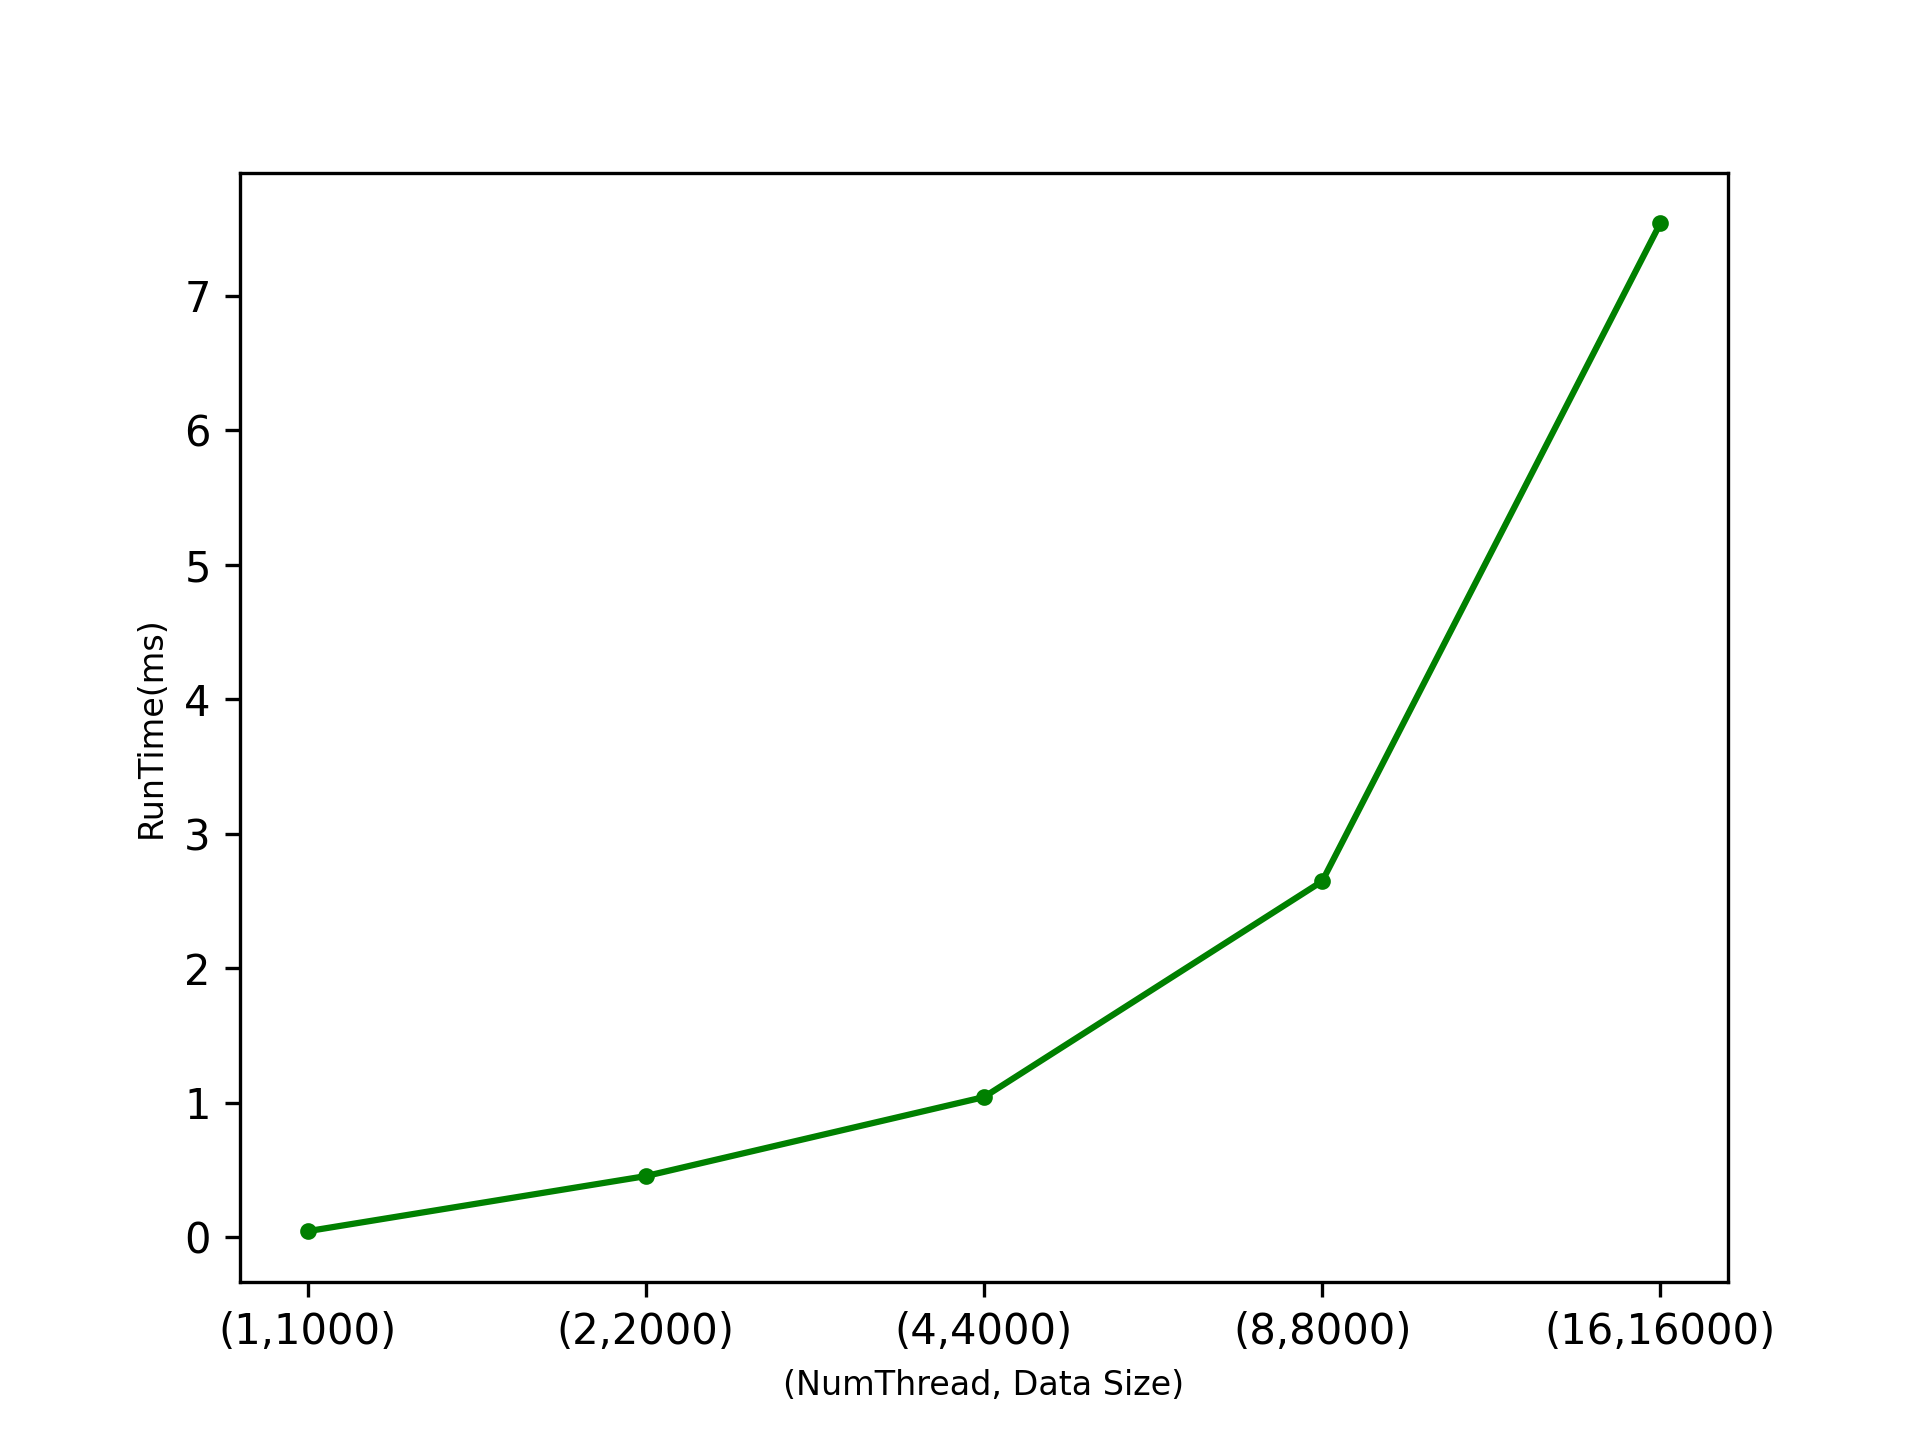
\includegraphics[width=.5\linewidth]{../figs/WeakScaling2_AllinOne.png}  
      \label{fig:WeakScaling2}
    \end{subfigure}
    \caption{Weak Scaling with balanced mode(left:Reduction, right: critical)}
    \label{fig:WeakScaling}
    \end{figure}
Figure \ref{fig:WeakScaling} shows the weak scaling of the program based on balanced mode.
Theoretically, when the problem size and thread number are both doubled, the runtime of the program should stay the same.
But we can see in the figure that the runtime of both version still increase. So both critical and reduction do not scale well, if we have to compare them,
the runtime of reduction version only doubled between (1,1000) and (16,16000), but for the critical version, it's around 10 times, so \textbf{we may conclude that reduction
version scales better.} The reason why it is so is mentioned above, the critical version act like the serial version but with much more additional
overhead caused by thread create and thread communication.

\subsection{Problems and Thinkings}

1. A problem we met is when we try to calculate the runtime of the function, if we just call the serial version without doing anything else,
then no matter how large the number we set to precision, the runtime of the serial version is always the same. We suspect that it's because the compiler
first calculate the result and embedded it into the binary program since it's just a simple function which do some easy mathmatic calculation and returns the same value everytime we call it, but we can't prove it.\\

2. The highest speedup we achieve is around 18.136 while the thread number is 28 and the data size is 56000 using reduction. Why the performance is so far away from the theoretical performance,
One reason may be the communication between threads and the overhead to create threads are too expensive; On the other hand, the overhead to access a data in other socket within NUMA system may also be costly.
\section{STREAM benchmark (2P)}
\subsection{Different sub-benchmarks}
There are 4 sub-benchmarks in STREAM \cite{stream01} as follows:
\begin{itemize}
  \item COPY: Copy from one array to another array. The benchmark measures transfer rates in the absence of arithmetic.
  \item SCALE: In addition to COPY, a simple arithmetic operation (multiply with a scalar) is added.
  \item SUM: Sum two arrays element-by-element and store the result to a third array. This requires envolving a third operand, thus multiple load/store ports of the processor can be tested.
  \item TRIAD: In addition to SUM, a scalar-multiplication is added. This allows to test chained/overlapped/fused multiply/add operations.
\end{itemize}

\begin{center}
  \begin{tabular}{ c|c } 
    Name & Code \\
    \hline
    COPY & $a[i] = b[i];$ \\
    SCALE & $a[i] = s*b[i];$ \\
    SUM & $a[i] = b[i]+c[i];$ \\
    SUM & $a[i] = b[i]+s*c[i];$ \\
  \end{tabular}
\end{center}
\textit{* a, b, c are vectors while s is a scalar.} \\
\subsection{STREAM version}
We used the STREAM version which distributed by Intel\cite{stream02}. This version has the same source code (stream.c) as the original version. The difference is there are some compiler optimisations flags, which is:
\begin{itemize}
  \item Flag for Vectorization: -xCORE-AVX2
  \item Cache bypass - Optimisation for data store: -qopt-streaming-stores always
  \item Common optimisation flags: -Wall -O3 -mcmodel=medium -shared-intel -qopenmp
\end{itemize}

\subsection{Benchmark on single core of Haswell}
\subsubsection{Array size}
According to the instruction, the $STREAM\_ARRAY\_SIZE$ should be at least 4x the size of the last level cache in the system. L3 cache of Xeon E5-2697 has 17920K, thus we chose $STREAM\_ARAY\_SIZE=10000000$.
\subsubsection{Results}
\begin{lstlisting}[frame=single]
  Function    Best Rate MB/s  Avg time     Min time     Max time
  Copy:           21365.3     0.007128     0.006871     0.007564
  Scale:          20465.5     0.007406     0.007173     0.007831
  Add:            21982.4     0.010295     0.010017     0.010664
  Triad:          22104.4     0.010281     0.009962     0.010696
\end{lstlisting}

\subsection{Benchmark on different cache levels}
According to the instruction, when one wants to measure the memory bandwidth, the $STREAM\_ARRAY\_SIZE$ should be at least 4 times larger than the lowest cache level. Following the same logic, we need to have $STREAM\_ARRAY\_SIZE$ 4 times larger than L2 cache if we want to measure the bandwidth between L2 and L3, 4 times larger than L1d for measuring bandwidth between L1d and L2.  

Besides, we need to make sure that cache-bypass is disable so that caches are used to store data, and memcpy() is disable. For that, we used the flags $-qopt-streaming-stores never -fno-builtin$.

The Figure \ref{fid:stream1} show the memory throughput respect to different array size. 
\begin{figure}[htpb]
    \centering
    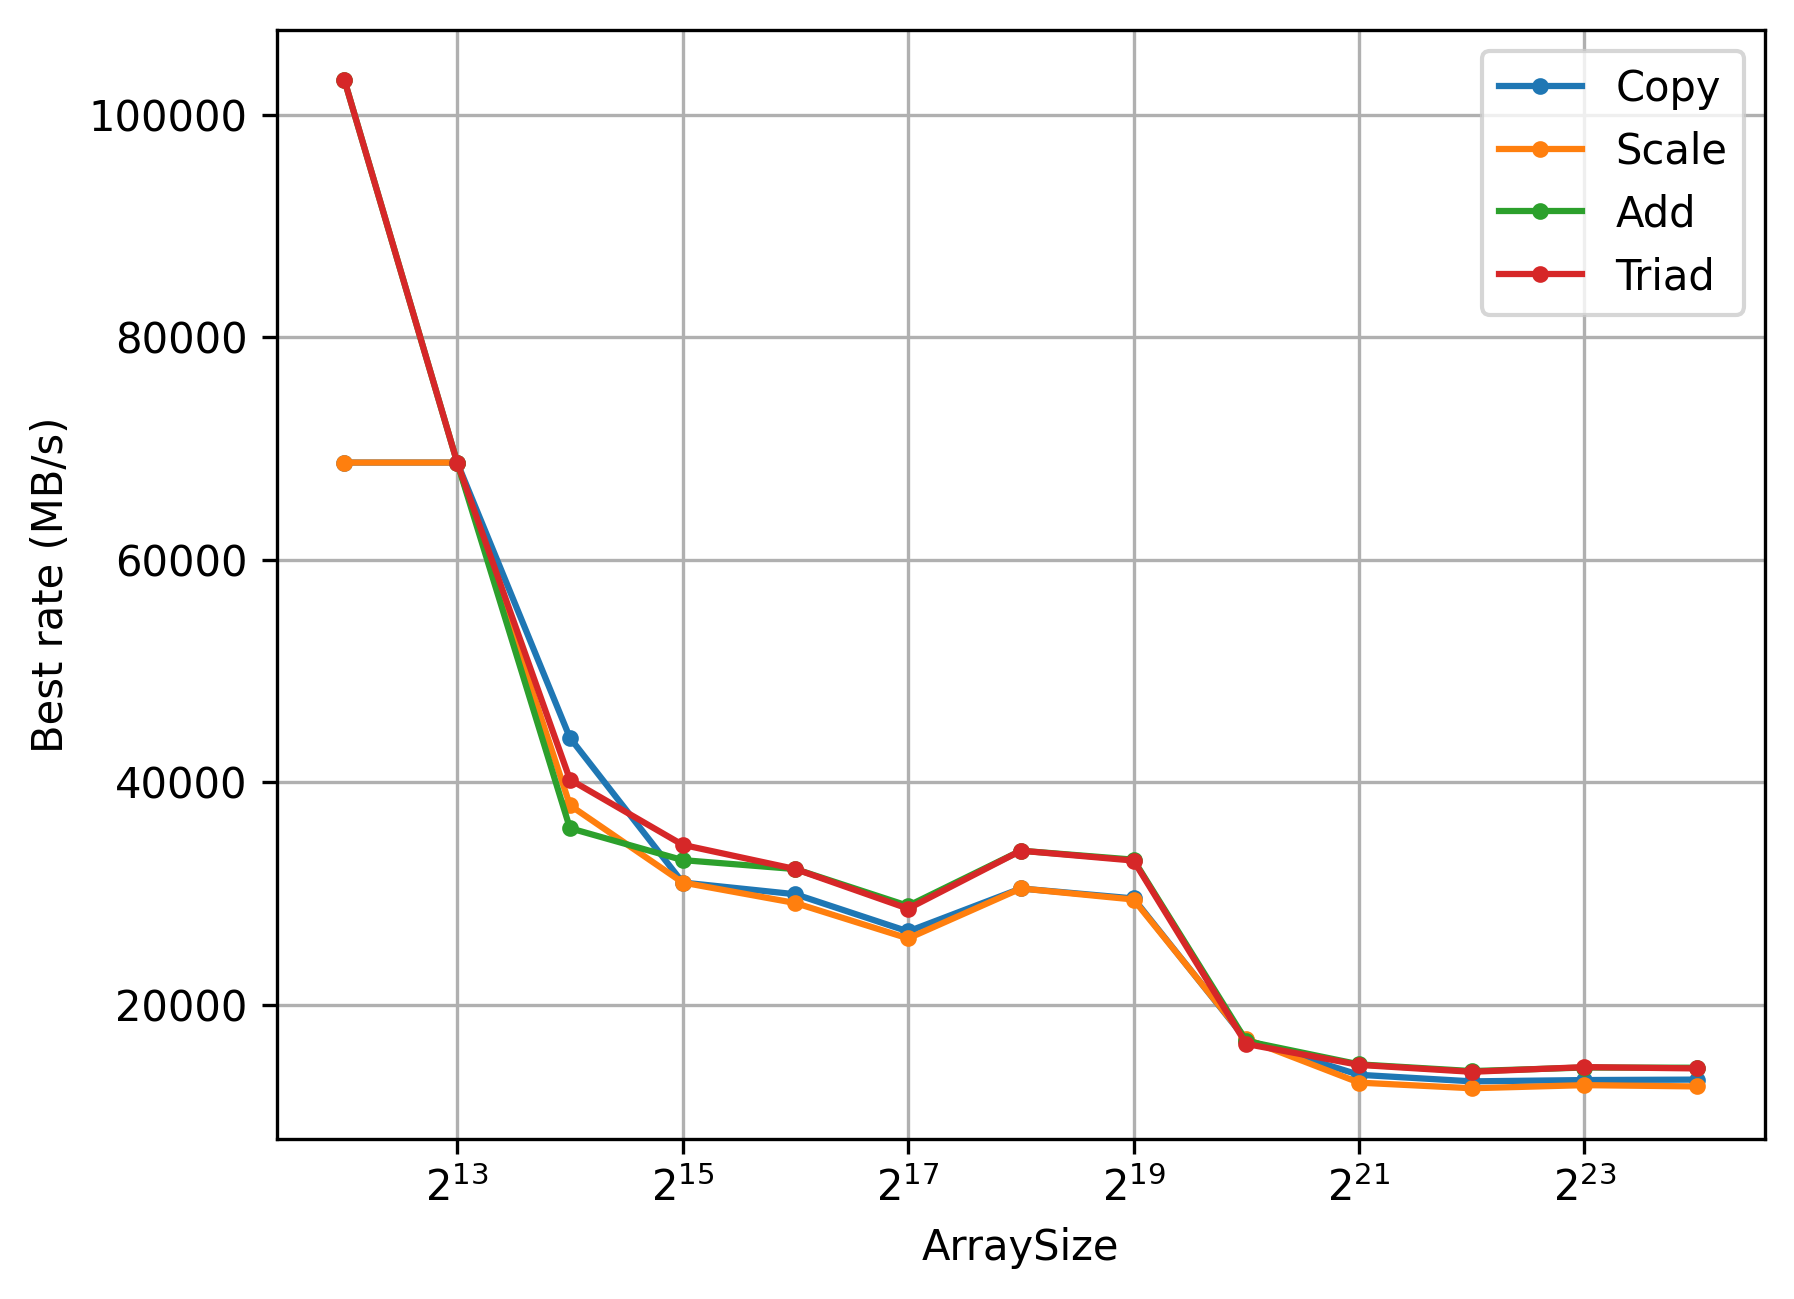
\includegraphics[width=\textwidth,height=8cm,keepaspectratio=true]{../figs/2.4_StreamCaches.png}
    \caption{Memory Throughput vs. Array Size}
    \label{fig:stream1}
\end{figure}

The memory through of different cache levels are presented in the table below:
\begin{center}
  \begin{tabular}{ c|c|c|c|c } 
    Array Size & Copy (MB/s) & Scale (MB/s) & Add (MB/s) & Triad (MB/s) \\
    \hline
    4096    & 68719.5&         68719.5&         103079.2       & 103079.2 \\
    8192    & 68719.5&         68719.5&         68719.5        & 68719.5 \\
    16384   & 43980.5&         37914.2&         35853.6        & 40226.0 \\
    32768   & 30972.2&         30972.2&         32985.3        & 34359.7 \\
    65536   & 29918.7&         29126.1&         32180.8        & 32180.8 \\
    131072  & 26574.3&         25947.2&         28871.2        & 28620.7 \\ 
    262144  & 30436.3&         30436.3&         33831.1        & 33831.1 \\
    524288  & 29541.9&         29443.0&         33026.6        & 32944.2 \\
    1048576 &         16810.5        & 16895.3       &  16722.6&         16459.2\\
    2097152 &         13690.4        & 12985.6       &  14626.6&         14580.2\\
    4194304 &         13099.8        & 12478.4       &  14023.7&         13957.9\\
    8388608 &         13217.0        & 12759.5       &  14343.6&         14381.5\\
    16777216&         13258.0        & 12641.2       &  14324.2&         14259.8\\
  \end{tabular}
\end{center}

L1d size is 32K which can store 4096 elements. From the benchmark results, one can see that the memory bandwidth of L1d - L2 is around ~67 GB/s. L2 size is 256K which is 32768 elements, then the memory throughput of L2 - L3 is around ~29 GB/s. L3 size is 17920K which is around 2,3 million elements, then the memory bandwidth of L3 - Memory is around ~13 GB/s. The L3- Memory bandwidth is way smaller than the maximum bandwidth of the system, since we ran the test on only 1 core, thus could not ultile/saturate all memory channels/lanes the system has. For the L1d-L2 and L2-L3 bandwidth, we could not find the maximum bandwidth from the Intel specification.

\subsection{Benchmark on a full node with OpenMP}
On each node on cm2, we have 4 NUMA nodes, in each node 7 cores share the same L3 cache which is 17920K in size. Thus, when running this benchmark on a fully single node system, we need to have the array size at least 4*4 times larger than 1 single L3 size. Thus, we chose $40000000$ as a size of $STREAM\_ARRAY\_SIZE$. 
We used the default setting for $KMP\_AFFINITY=granularity=thread,compact,1,0$

The result is presented in the Figure below:
\begin{figure}[htpb]
    \centering
    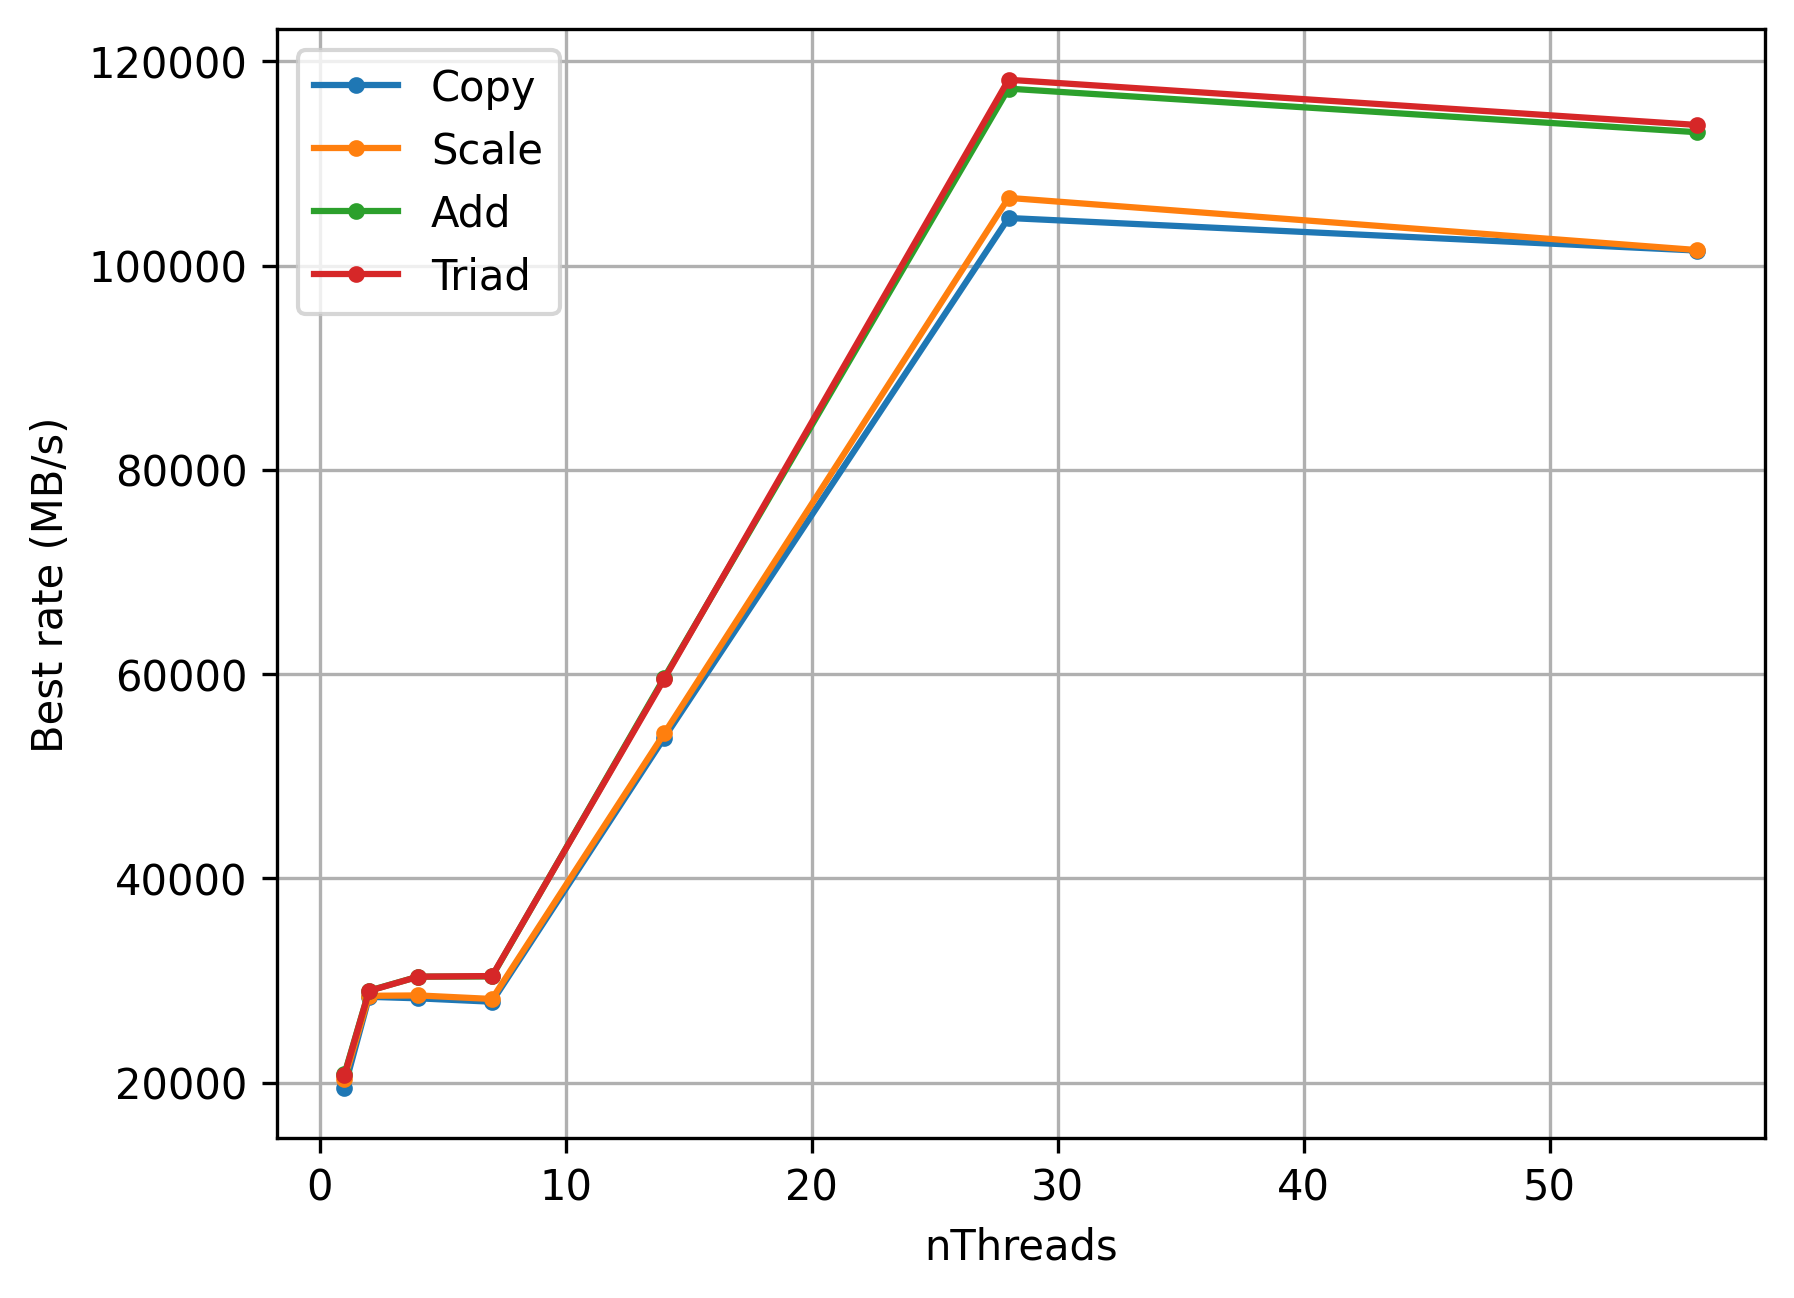
\includegraphics[width=\textwidth,height=8cm,keepaspectratio=true]{../figs/2.5_StreamScale.png}
    \caption{STREAM with size=40000000, respect to nThreads}
    \label{fig:stream2}
\end{figure}
For a single core, the rate stays around 20000MB/s. For the case when we have 2-7 cores, the throughput stay steadily around 30000MB/s, does not change much. This can be explain by looking at the processor topology. For Haswell, each 7 cores are packed together into 1 block and all cores share the same L3 cache, this block then connects to the main memory through some lanes. When the number of threads increases from 1 to 2,4, or 7, it still stays in the same blocks, thus the utilised number lanes still stay the same, thus no big changes in the memory throughput. From the figures, we can see that when the nThreads increase from 7 to 14, or 14 to 28, the memory throughput increases by 2 or 4 times very nicely, respectively. This is because we moved from 1 core block to 2 or 4 blocks, leading to the number of lanes increasing by 2 or 4, resulting in double or 4x memory throughput. When the number of Threads increase from 28 to 56, there is a slightly drop in performance. This is understandable since the system has only 28 cores physically with 2 threads per cores. Increasing the number of threads to 56 does not increase number of lanes, but causing overloading the cores.
The peak bandwidth is at 118198 MB/s which is ~115.5 GB/s. According to Intel specification, Haswell E5-2697 vs has maximum bandwidth as 68 GB/s. Since each node has 2 processors, then the maximum bandwidth is 136 GB/s. The measured bandwidth is 85% of the maximum bandwidth which is pretty good.
\subsection{Effect of NUMA to the STREAM benchmark}
In this task, we try to compare the performance of STREAM with and without First-touch optimisation. For the test without First-touch, we initialized data ( for all a,b, and c vectors) in a single thread. For the test with First-touch, we initialized data in a parallel with \textit{pragma omp parallel for}. By default, the schedule strategy is static and the chunksize equal to the number of iteration devide by number of threads. The performance comparison is presented in the figure below:
\begin{figure}[htpb]
    \centering
    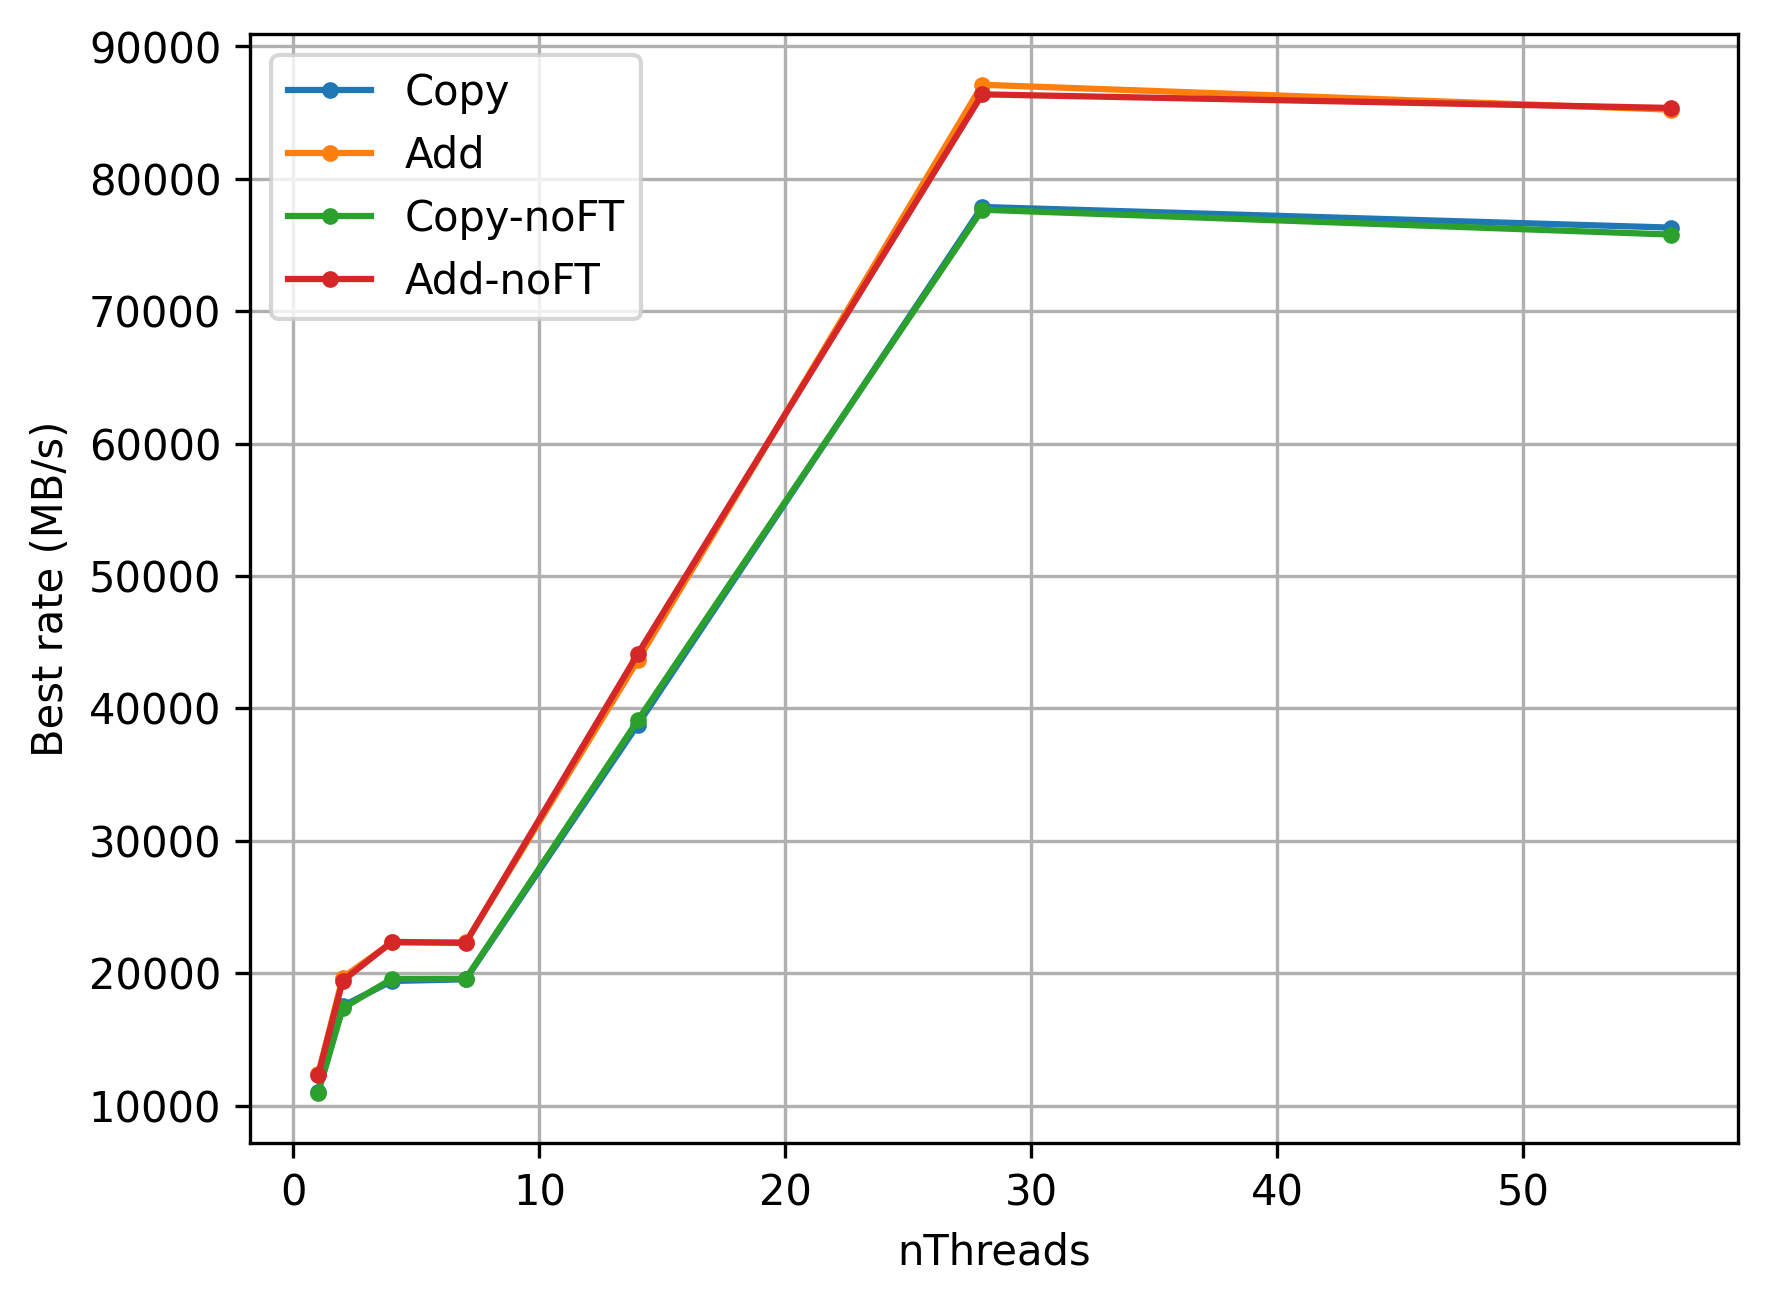
\includegraphics[width=\textwidth,height=8cm,keepaspectratio=true]{../figs/2.6_StreamCompare.png}
    \caption{Comparison between Performance of Stream with and without First Touch Optimisation}
    \label{fig:stream1}
\end{figure}
We used the default setting for $KMP\_AFFINITY=granularity=thread,compact,1,0$
It's surprising that there are no big difference in performance in the two test. One would expect to have the same performance only for the case when nThreads equals 1,2,4,7, and as soon as nThreads is larger then 7, performance of the one without first-touch optimisation will be worst because of NUMA issues. However, we could not observe the effect here.



\section{Quicksort (2P)}
\subsection{Code}
\begin{lstlisting}[frame=single]
void quicksort(double *data, int length, int num_thread)
{
  ...
#pragma omp task default(none) shared(data, num_thread) \
                   firstprivate(right)\ 
                   final(right < array_length/num_thread)
  quicksort(data, right,num_thread);
#pragma omp task default(none) shared(data,num_thread)\ 
                 firstprivate(length, left)\ 
                 final(length - left < array_length/num_thread)
  quicksort(&(data[left]), length - left,num_thread);
#pragma omp taskwait
  ...
}
int main()
{
  ...
#pragma omp parallel
  {
    #pragma omp single // Only one thread should create tasks
    quicksort(data_cpy, length,omp_get_max_threads());
  }
  ...
}
\end{lstlisting}

\subsection{Evaluation}
\begin{figure}[ht]
    \centering
    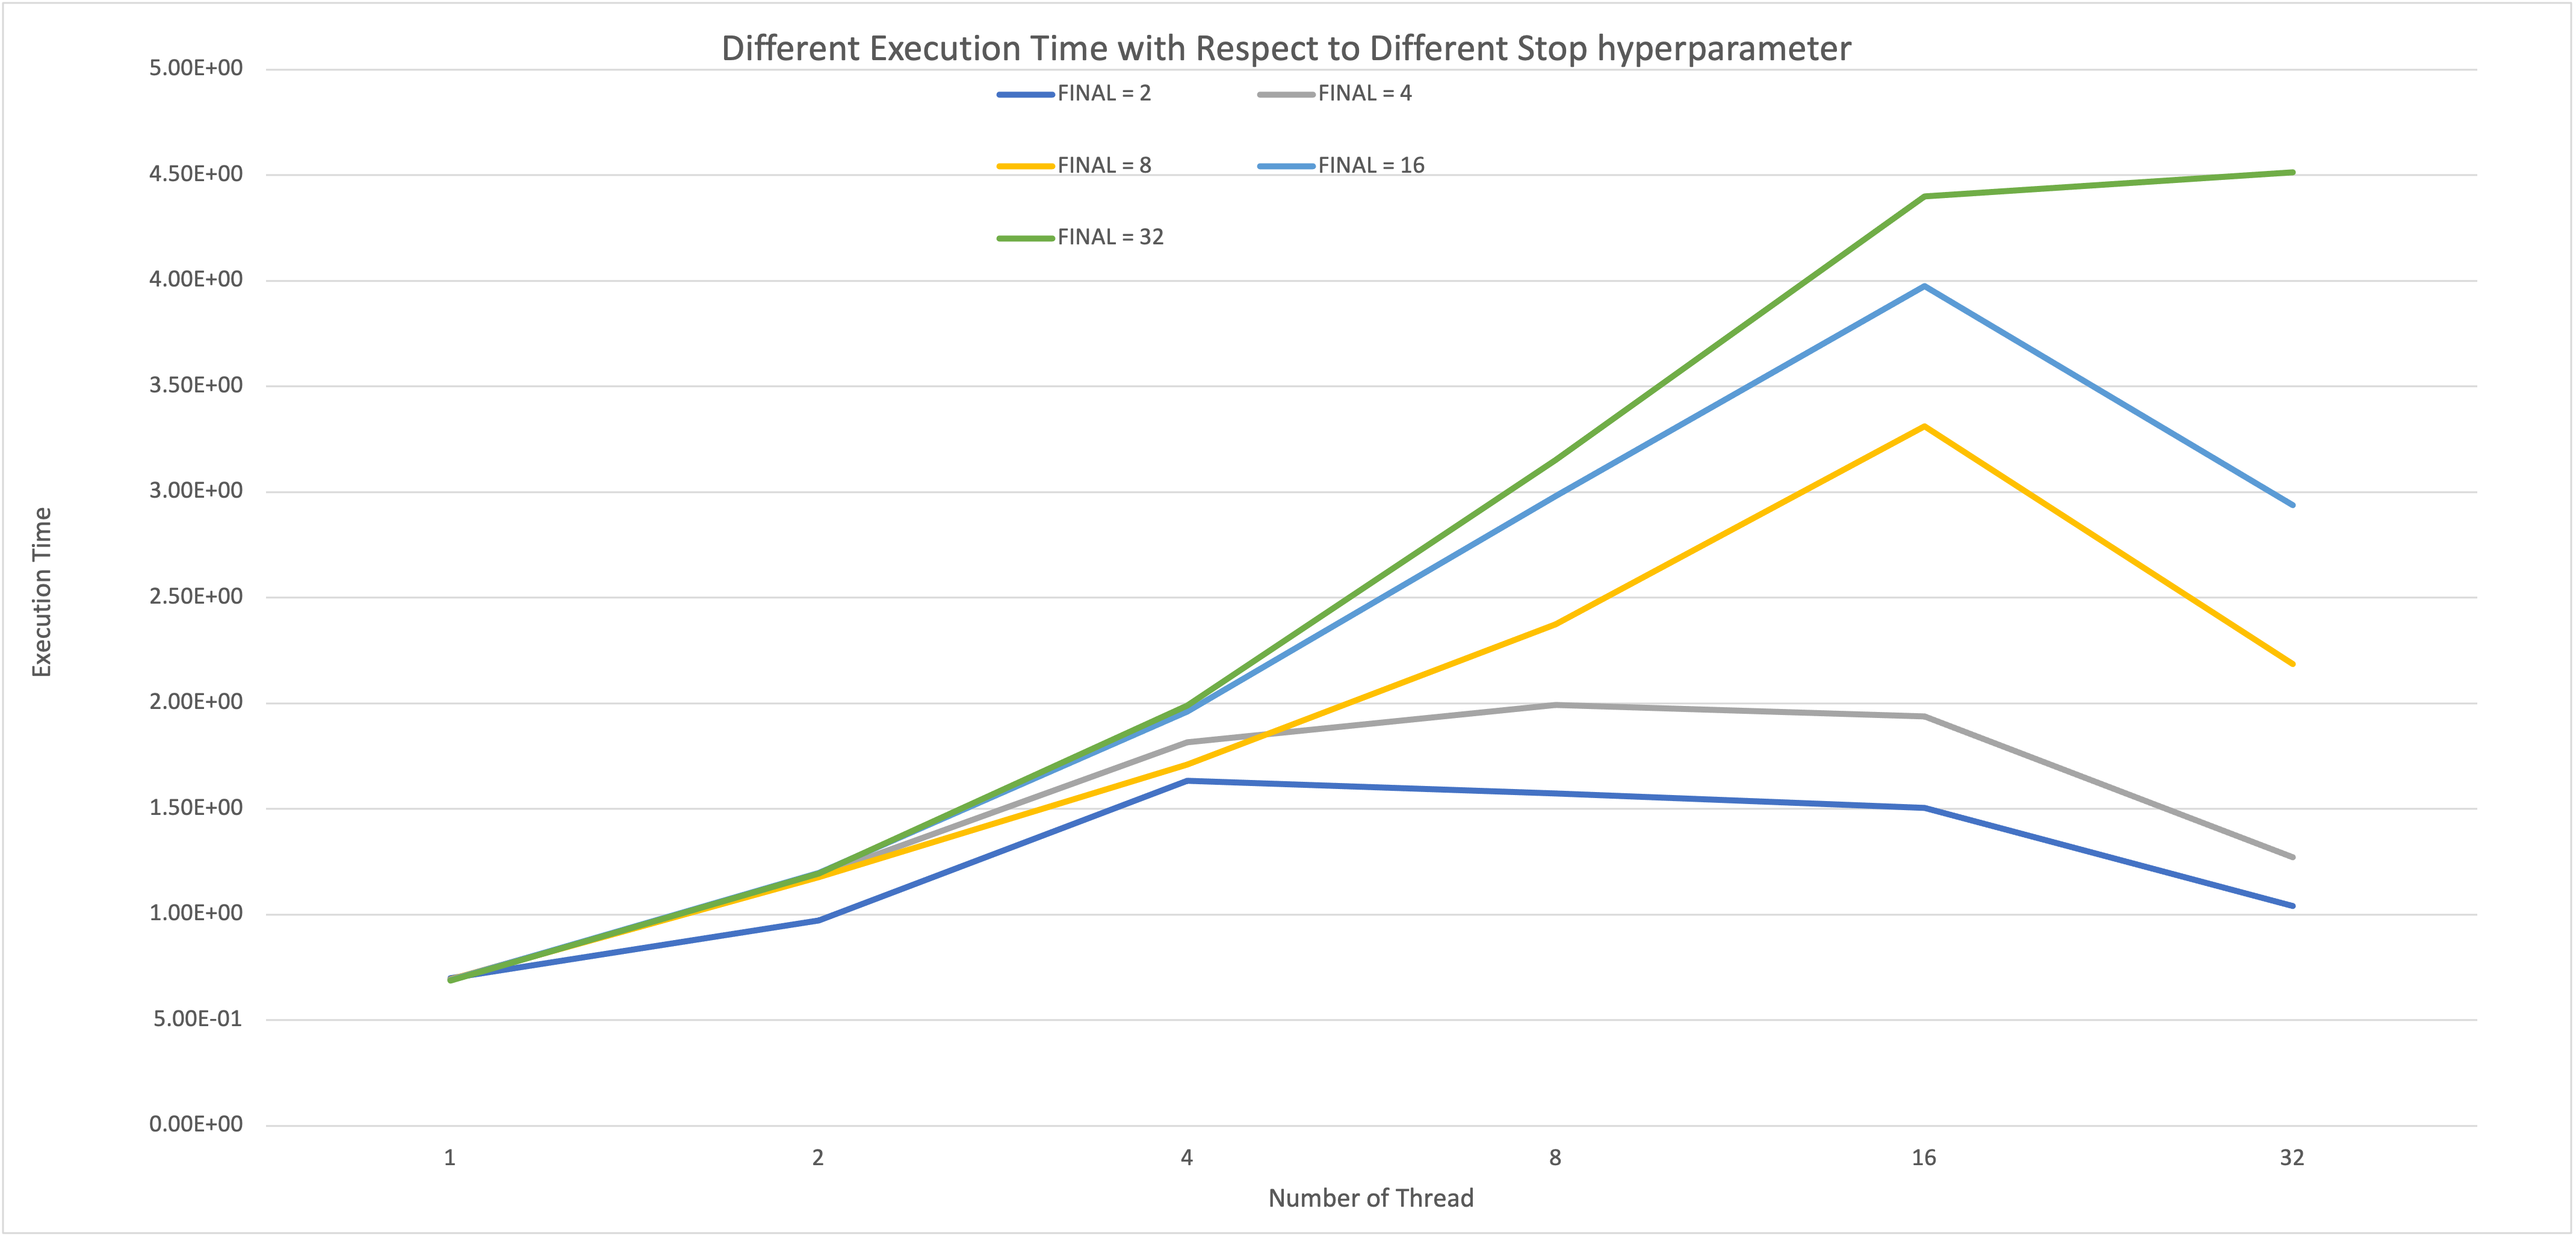
\includegraphics[width=.99\linewidth]{../figs/Final_hyper.png}  
    \label{fig:final_hyper}
    \caption{Strong Scaling with Different Stop Condition}
\end{figure}
We first run our program with different Stop Condition to find the best hyperparameter for our program.
As shown in Figure \ref{fig:final_hyper}, we set the stop condition to different FINAL,
namely, $final(subArrayLength \textless arrayLength/FINAL)$, and we find out that $FINAL = NUM\_THREAD$ can give us a good performance in most cases.\\
\begin{lstlisting}[frame=single]
# Overhead      Pid:Command  
# ........  .................
#
     3.73%    24111:quicksort
     3.57%    24125:quicksort
     3.57%    24129:quicksort
     3.57%    24128:quicksort
     3.57%    24132:quicksort
     3.57%    24112:quicksort
     3.57%    24122:quicksort
     3.57%    24117:quicksort
     3.57%    24119:quicksort
     3.57%    24120:quicksort
     3.57%    24135:quicksort
     3.57%    24137:quicksort
     3.57%    24138:quicksort
     3.57%    24114:quicksort
     3.57%    24130:quicksort
     3.57%    24127:quicksort
     3.57%    24126:quicksort
     3.56%    24134:quicksort
     3.56%    24123:quicksort
     3.56%    24116:quicksort
     3.56%    24113:quicksort
     3.56%    24115:quicksort
     3.56%    24124:quicksort
     3.56%    24118:quicksort
     3.56%    24136:quicksort
     3.56%    24121:quicksort
     3.56%    24133:quicksort
     3.56%    24131:quicksort
\end{lstlisting}

Also, we recorded our program using the thread number as the final parameter, and the result above shows us a quite good workload.

\begin{figure}[htpb]
  \centering
  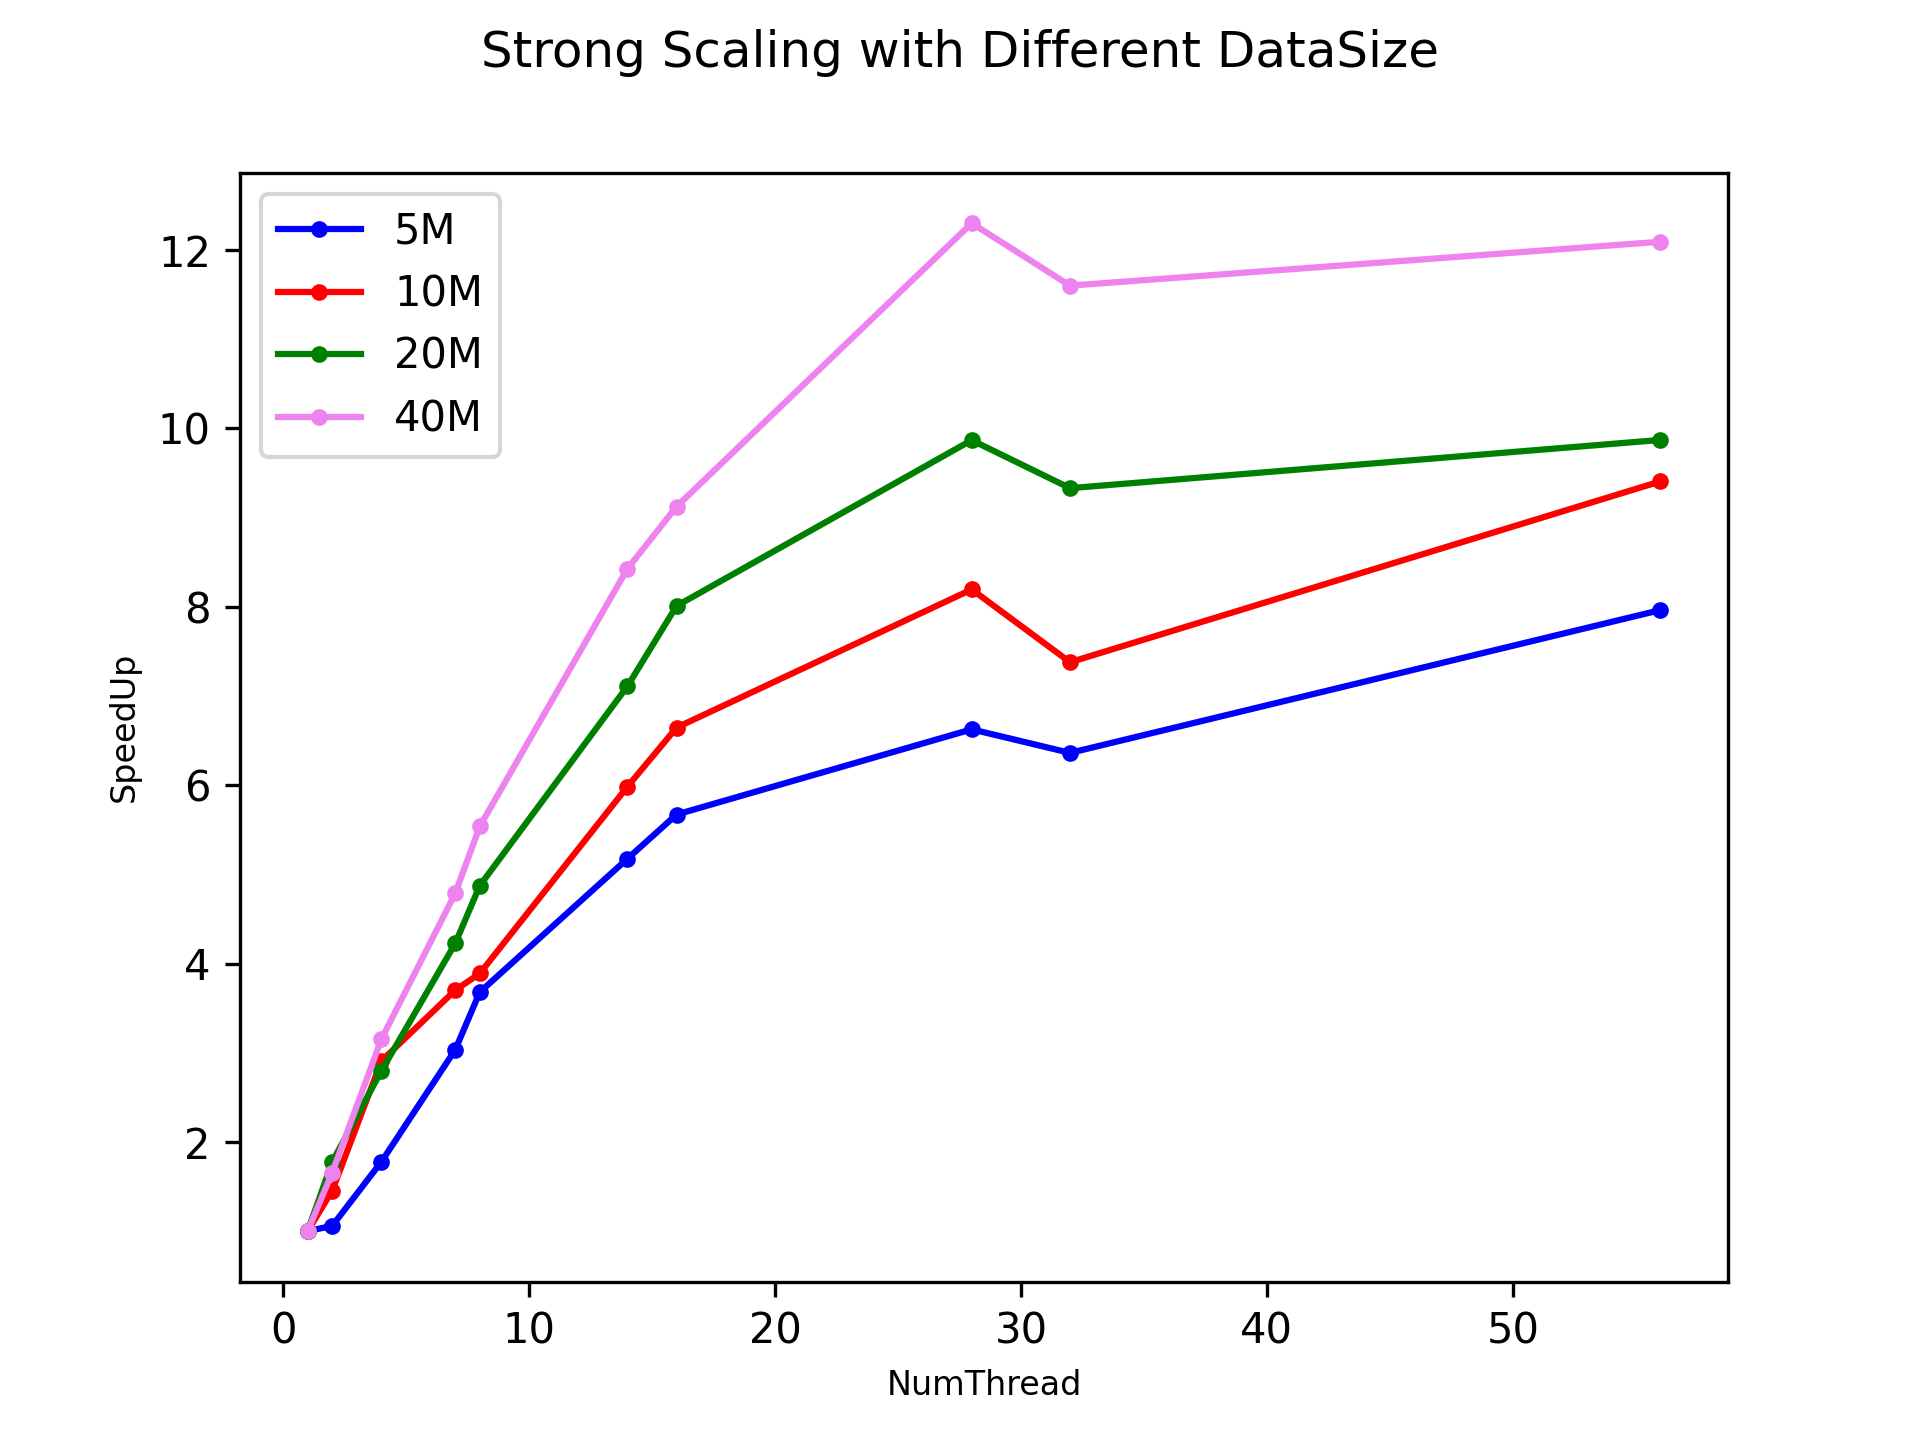
\includegraphics[width=.8\linewidth]{../figs/quicksort_strongscaling.png}  
  \label{fig:quicksort}
  \caption{Strong Scaling with different Data Size}
\end{figure}

Based on the result above, we then evaluate the strong scaling of our program using balanced mode. As shown in Figure \ref{fig:quicksort},
Our program scaled quite good except from the part 28 threads to 56 threads which is again the hyperthread problem we mentioned above.

\subsection{Thinkings}
The performance we achieve in this program is actually not so good as the theoretical speed up should be 28. We tried to optimize our code by implementing first touch policy,
but we can't find a proper way since the array is randomly generated and we can't know how many tasks will be generated in advance.
But since the best performance in Question1 is around 18 and it's a much simpler program, we guess it's just because the use of openmp causes many overheads.
\\
\\
\section{Matrix-Matrix-Multiplication (4P)}

As in the Assignment 1, we followed the algorithm introduced in Fig. 8 of \cite{Goto08}. The choice of submatrix dimessions stay the same as our choice in Assignment 1, since it gave the best performance for microkernel, so does other higher level kerners. 

\begin{center}
    \begin{tabular}{|c |c| c| c | }
        \hline
        $m_c$ & $k_c$ & $m_r$ & $n_r$ \\
        \hline
        32  & 64   & 32   & 2   \\
        \hline
    \end{tabular}
\end{center}

\subsection{OpenMP Implementation}
We used nested \textit{omp parallel for} loop as our main implementation.

The first \textit{omp parallel for} loop is implemented in $GEPP$ which creates $nTeams$ of thread teams, each thread team calls a $GEBP$ kernel with different data sets. All thread teams shared the same $B\_pack$. However, each thread teams have different $A\_pack$.  

The second \textit{omp parallel for} loop is implemented in $GEBP$ which creates $ThreadsPerTeam$ of threads. Each thread shares the same $A\_pack$, but have different B elements and C elements.

\subsection{OpenMP Optimisation}

\subsubsection{General Optimisations}
Inspired by \cite{openmp1}, we did some general optimisations for OpenMP as follows:
  \paragraph{Parallel Region Expansion:}
  We replaced two \textit{\#pragma omp parallel for} with one single parallel block. With this, we eliminate costs of initializing parallel area.\\
    \begin{minipage}{.49\textwidth}
      \begin{lstlisting}[caption=Before,frame=single]
#pragma omp parallel for \
   num_threads(nTeams)
for (int i=0; i < S; i++)
{
      ...
}
#pragma omp parallel for \
   num_threads(nTeams)
for (int i=0; i < S/MC; i++)
{
      ...
}
\end{lstlisting}
\end{minipage}\hfill
\begin{minipage}{.49\textwidth}
\begin{lstlisting}[caption=Expansion of parallel region,frame=single]
#pragma omp parallel \
   num_threads(nTeams)
{ // starting parallel region
   #pragma omp for
   for (int i=0; i < S; i++)
   {
      ...
   }
   #pragma omp for
   for (int i=0; i < S/MC; i++)
   {
      ...
   }
} // end parallel region
        \end{lstlisting}
        \end{minipage}
\paragraph{Barrier Elimination:}
We also eliminated a synchronisation point at the end of the second \textit{pragma omp for} with $nowait$ since the there is a synchronisation point after the first \textit{pragma omp for} which already enforces the correct results.

    \noindent\begin{minipage}{.70\textwidth}
%      \begin{minipage}{.45\textwidth}
        \begin{lstlisting}[caption=Barrier Elimination,frame=single]{Name}
#pragma omp parallel num_threads(nTeams)
{ // starting parallel region
   #pragma omp for
   for (int i=0; i < S; i++)
   {
   ...
   }
   #pragma omp for nowait
   for (int i=0; i < S/MC; i++)
   {
   ...
   }
} // end parallel region
        \end{lstlisting}
        \end{minipage}


\subsubsection{First-touch Optimisation}
To eliminate the problem with NUMA, we implemented First-touc policy. For this, we need to initialize data in 'parallel' so that the thread who works on a block of data later, also initialize that block, or at least that thread should stay in the same NUMA domain as the thread who initializes the block. We have different integration strategy for A, B, and C.

For A, since the threads in the same team read data from share the same block of $A\_pack$ which is copied from A, we just need to make sure that the master thread of the team is also initialize the block which their team works on. The initialization is as below:
\begin{lstlisting}[frame=single]
#pragma omp parallel for num_threads(nTeams) schedule(static)
    for (int j = 0; j < S/K; ++j) {
        for (int i = 0; i < S; ++i) {
            for (int jj = 0; jj < K; ++jj) {
                col = j*K + jj;
                A[col*S + i] = i + col;
            }
        }
    }
\end{lstlisting}

For B, since all thread teams work on the same $B\_pack$, instead of having only one $B\_pack$ shared among them, we created a array of $B\_pack$ so that each thread team can have their own $B\_pack$. With this, each thread team initialize their own $B\_pack$, and the memory page with stay within NUMA node, accessing to this local $B\_pack$ from all threads are 'UMA'. For initialization of B, since in each $GEPP$, all thread teams copied from the same B block to their own $B\_pack$, we initialized B in a cycle-columns based manner respect to number of thread teams. Initialization of B is found below:

\begin{lstlisting}[frame=single]
#pragma omp parallel for num_threads(nTeams)
    for (int j = 0; j < S; ++j) {
#pragma omp parallel for num_threads(threadsPerTeam)
        for (int i = 0; i < S; ++i) {
            B[j*S + i] = (S-i) + (S-j);
        }   
    }   

\end{lstlisting}

For C initialization, thread teams share row blocks, while threads in the same team share columns blocks.


\begin{lstlisting}[frame=single]
#pragma omp parallel for num_threads(nTeams) schedule(static)
    for (int i = 0; i < S/MC; ++i) {
#pragma omp parallel for num_threads(threadsPerTeam), schedule(static) 
        for (int j = 0; j < S/N; ++j) {
            for (int ii = 0; ii < MC; ++ii) {
                for (int jj = 0; jj < N; ++jj) {
                    C[(j*N+jj)*S + (i*MC+ii)] = 0.0;
                }   
            }   
        }   
    }   
#endif
\end{lstlisting}

All are scheduled with $static$ strategy and default chucksizes since the default chucksize work correctly respecting to the work-sharing later.
\subsection{Result and Discussion}
All the tests are with following configuration since it improves the performance for us:
\begin{lstlisting}
KMP_AFFINITY=granularity=core,balanced,1,0   
OMP_WAIT_POLICY=active                        
KMP_HOT_TEAMS=1                               
KMP_HOT_TEAMS_MAX_LEVELS=2                    
OMP_MAX_ACTIVE_LEVELS=2
\end{lstlisting}

The performance of the three tests $Kernelmicro$, $GEBP$, $GEMM$ are presented below:
\begin{figure}[htpb]
    \centering
    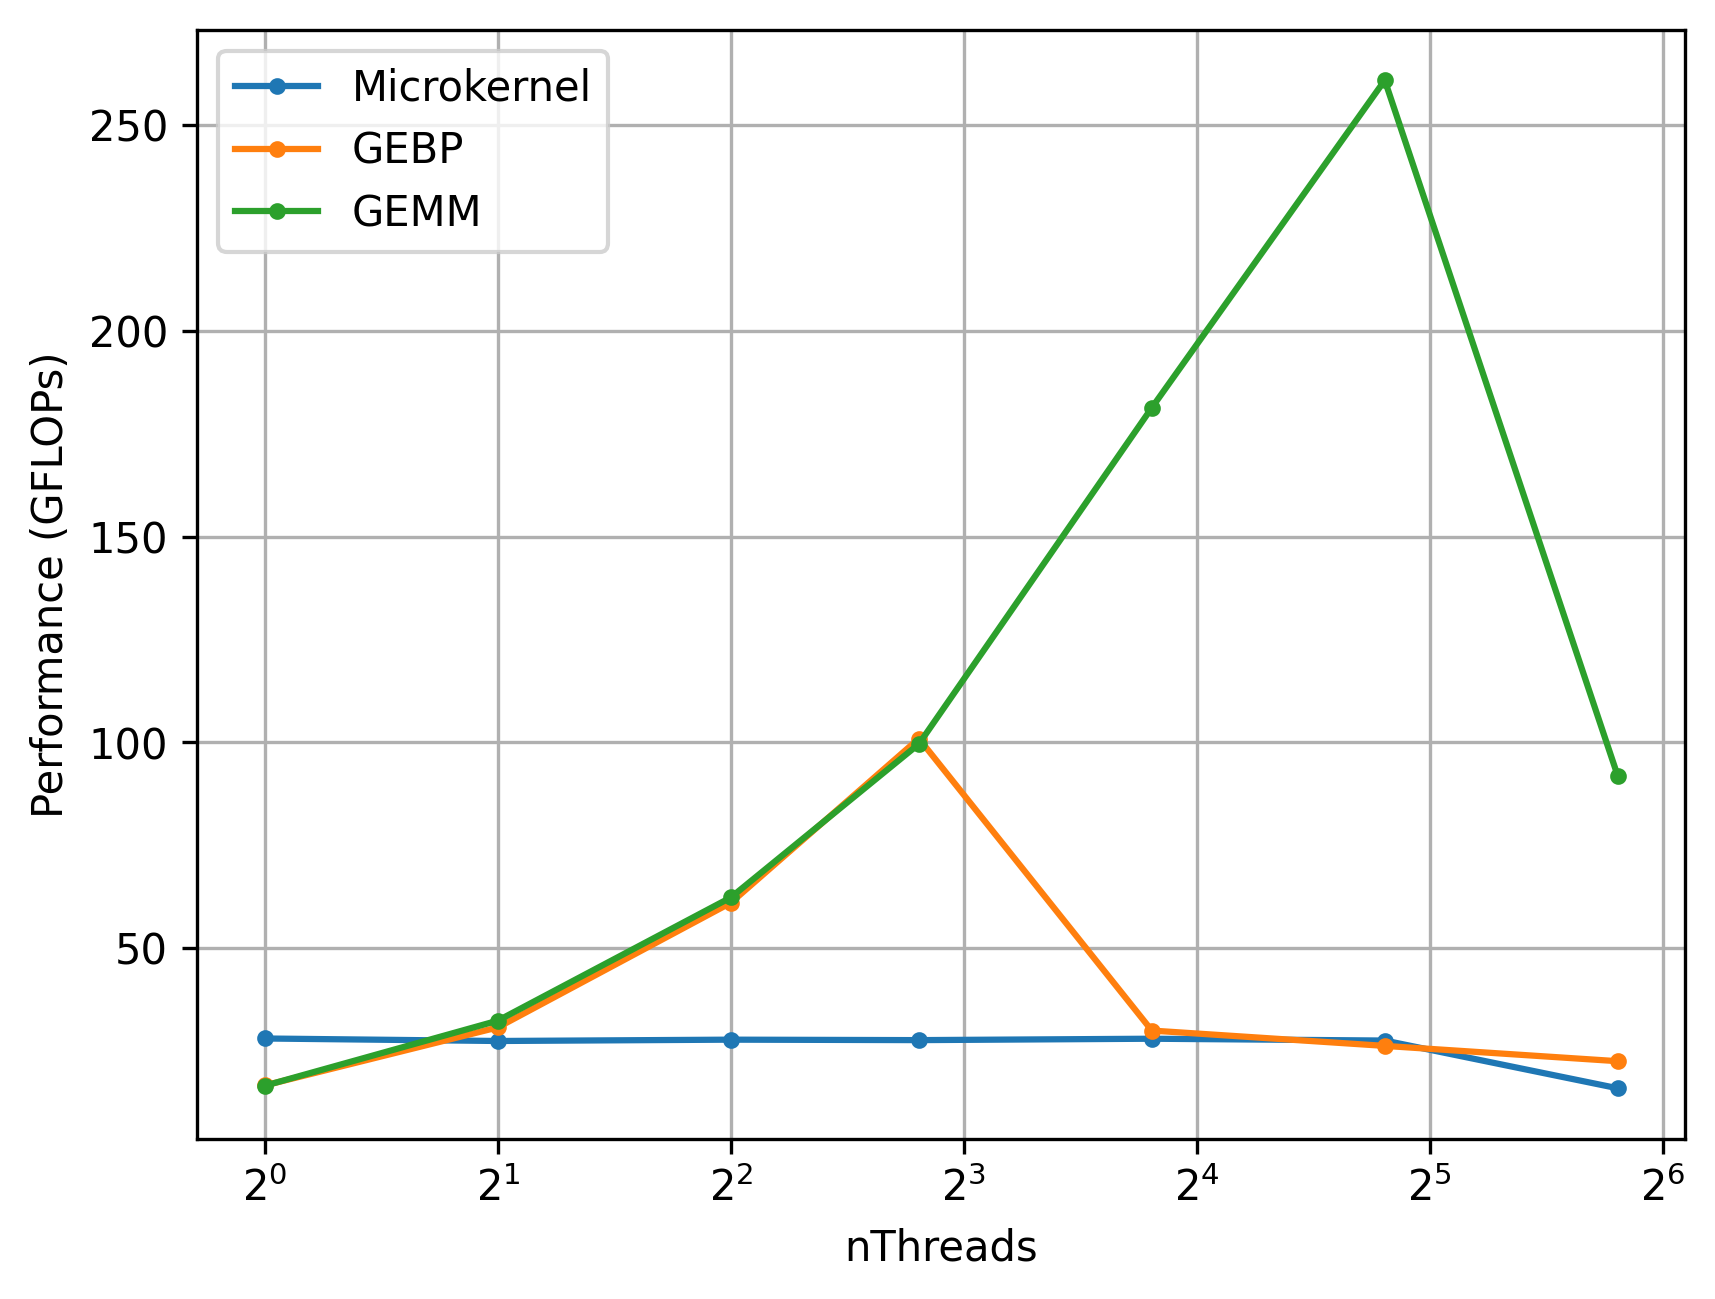
\includegraphics[width=\textwidth,height=8cm,keepaspectratio=true]{../figs/4.1_differenceTests.png}
    \caption{S=2048, Performance of different kernels}
    \label{fig:dgemm1}
\end{figure}
The performance of $Microkernel$ stays steadily around 27-28 GFLOPs during the scaling test, which is good. However, the performance of $GEBP$ reached a peak at ~100 GFLOPs with $nThreads=7$ at the droped down to 28 GFLOPs which is a bit weird. One might blame for NUMA problem, but taking account that we already implemented the First-touch and $GEMM$ also scale well even when nthreads larger than 7, then NUMA is the reason here. Lastly, as we already mention, $GEMM$ scales pretty well up to 28 threads, and drops down at 56 threads. This can be explained since we have only 28 cores on the system, when we use more then 28 threads, they are over-subscribed to the physical cores, affect negatively to the results, even though it has hyperthread.


We also tested with given 28 threads, how many number of thread teams or how many number of threads per team is the best. The result is presented below:
\begin{figure}[htpb]
    \centering
    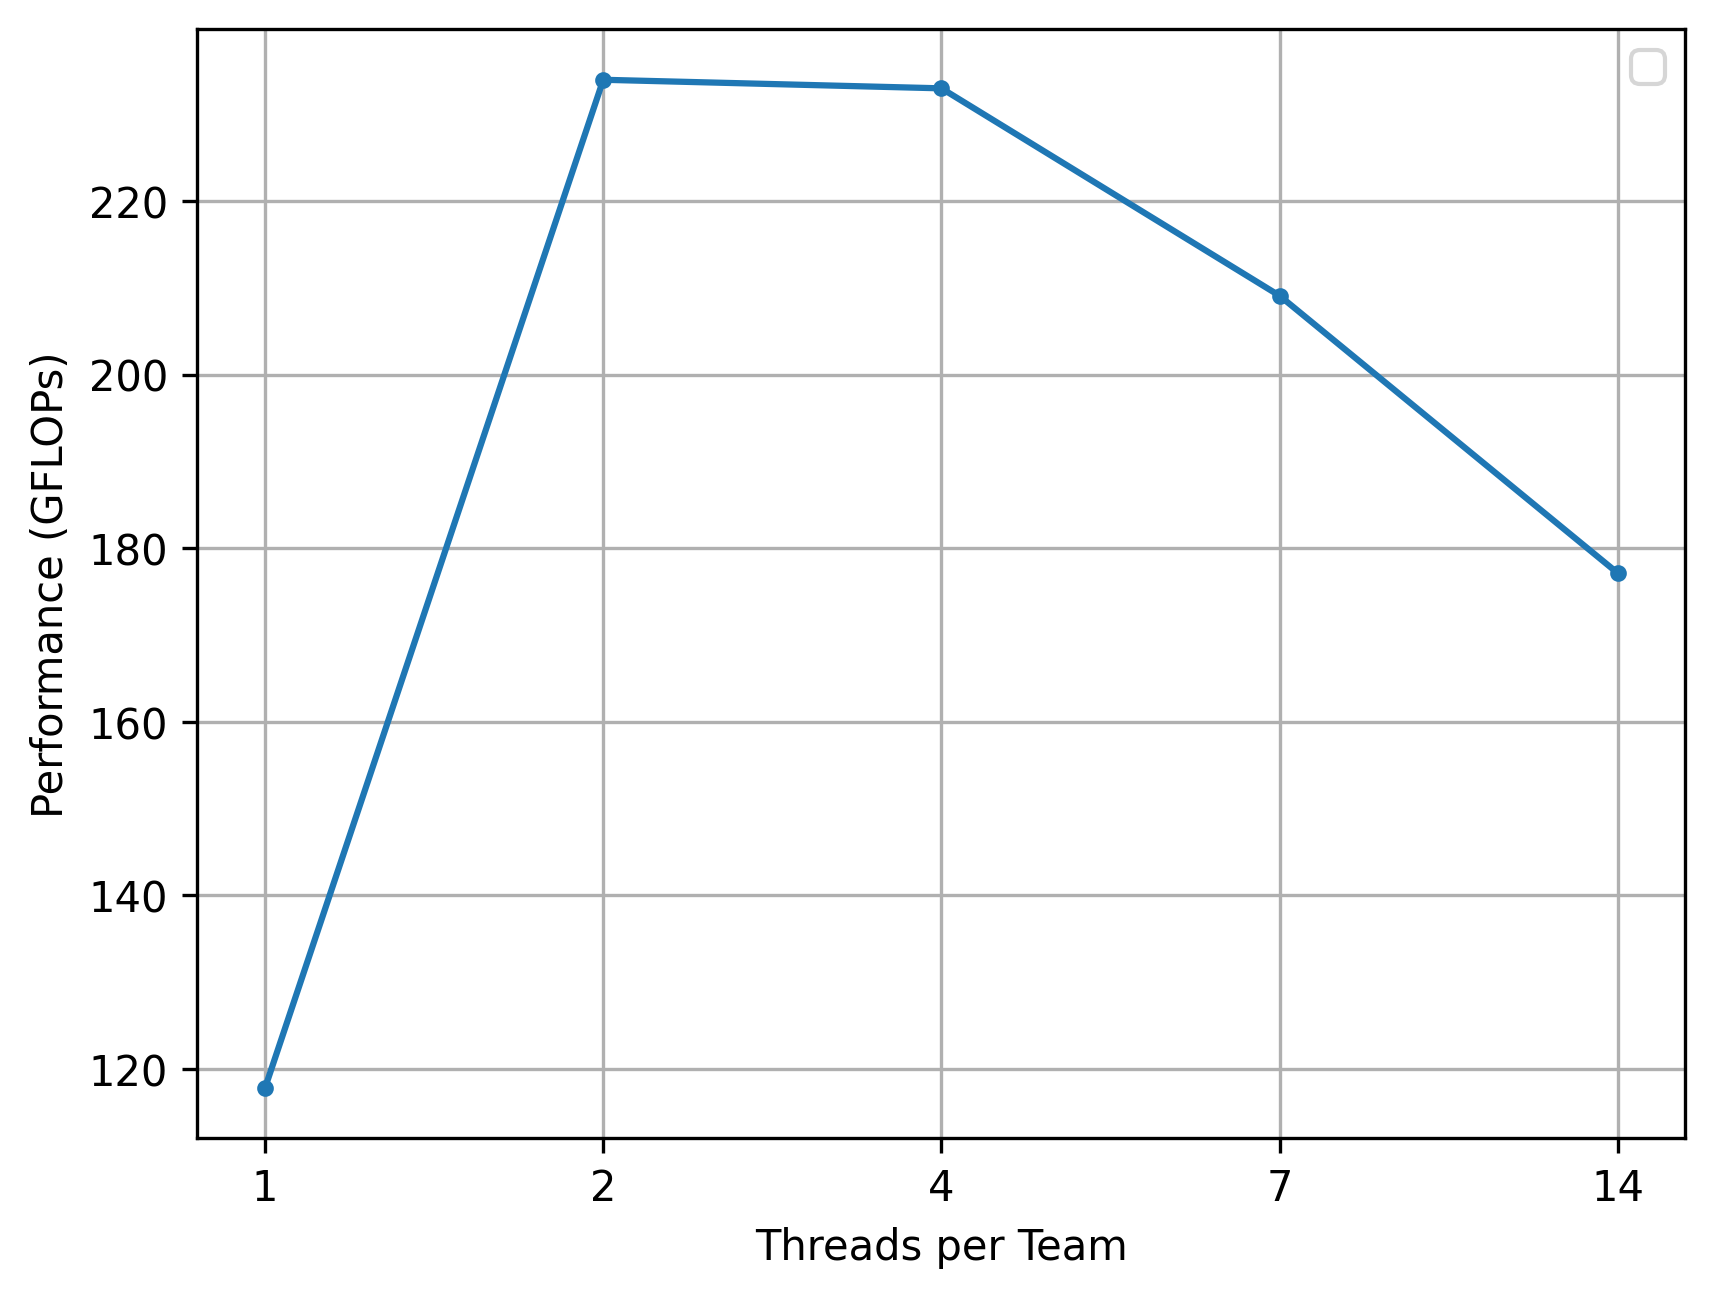
\includegraphics[width=\textwidth,height=8cm,keepaspectratio=true]{../figs/4.ThreadsPerTeam.png}
    \caption{S=2048, Performance of DGEMM with Different number of Threads per Team}
    \label{fig:dgemm2}
\end{figure}

So with 2 threads per team, the dgemm performs best. We will use this number for other tests from now.

The performance of with and without First touch Optimisation with 28 threads, 2 threads/team is prestend belows:


\begin{figure}[htpb]
    \centering
    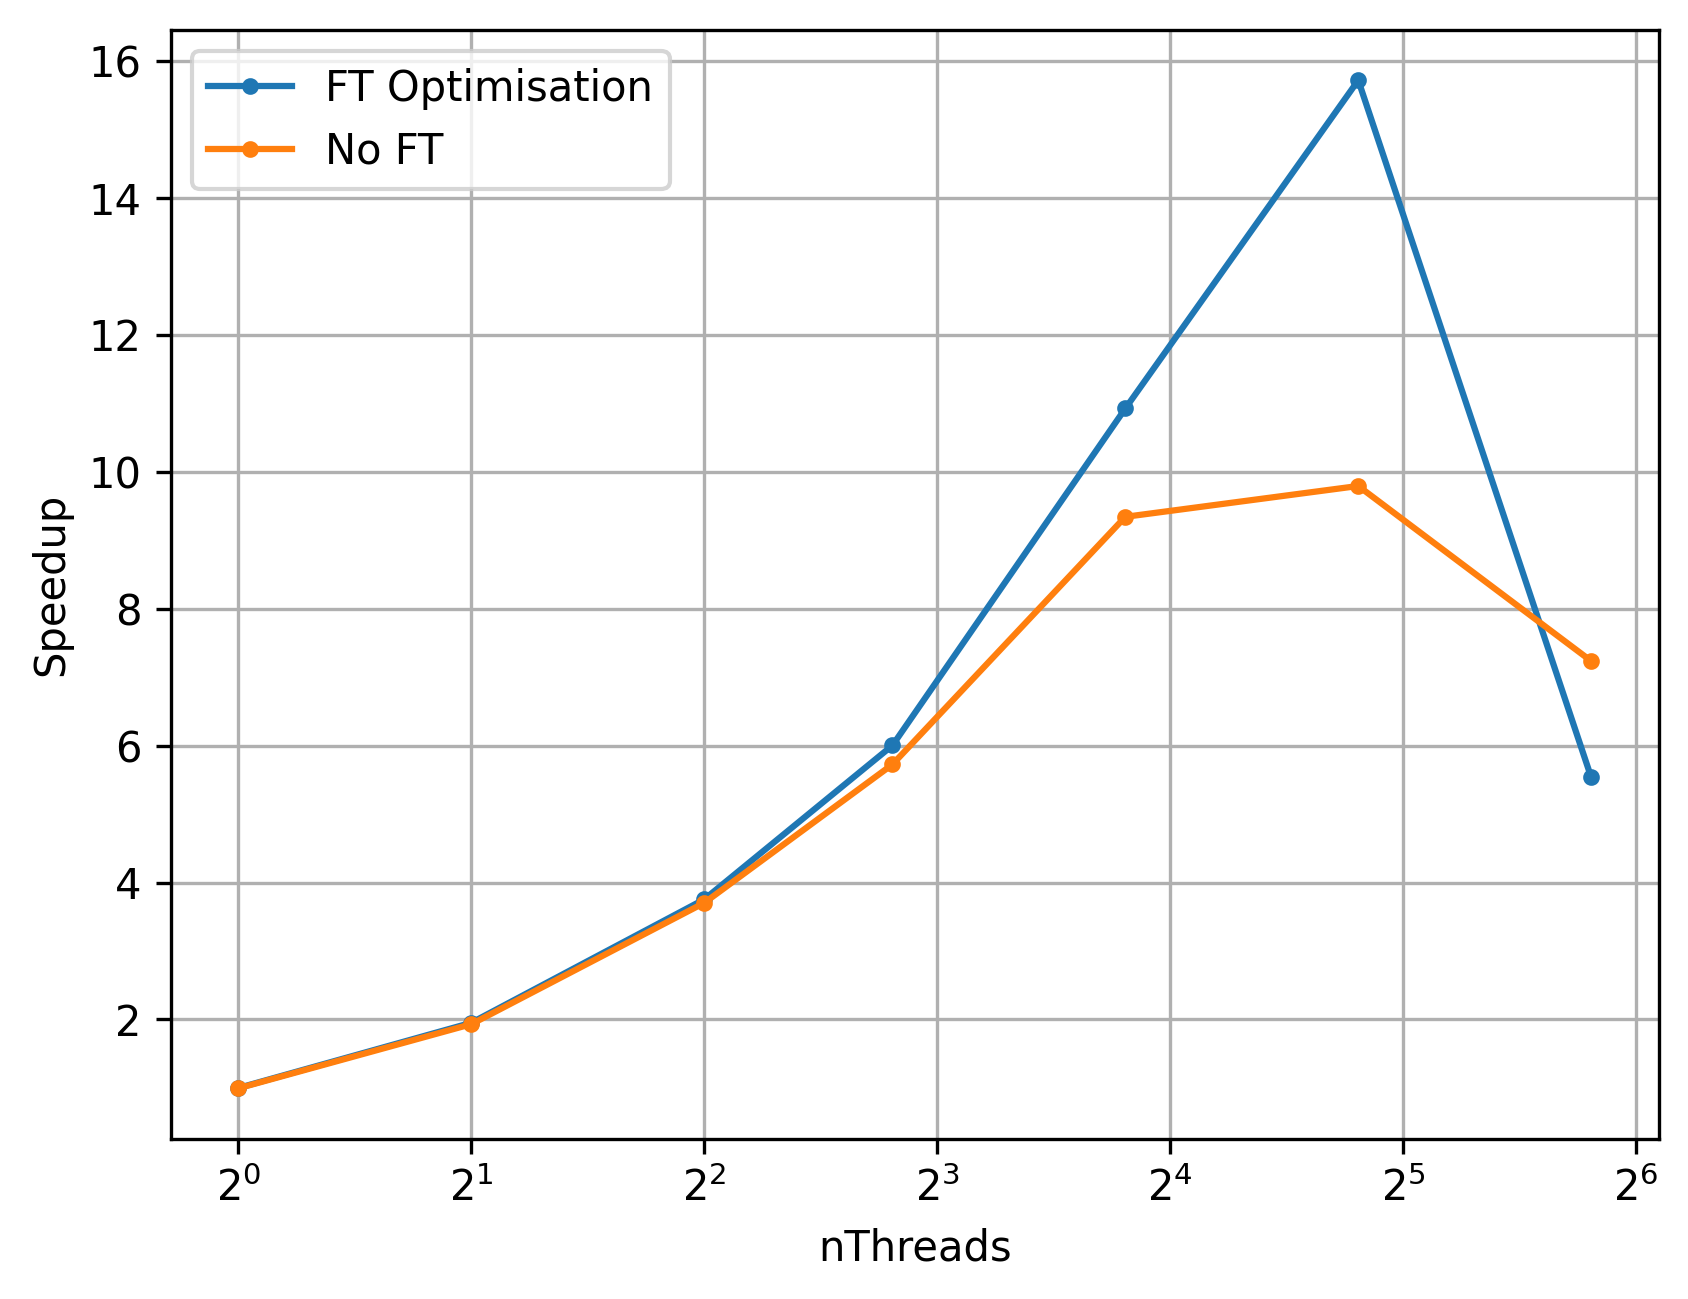
\includegraphics[width=\textwidth,height=8cm,keepaspectratio=true]{../figs/4.2_CompareNoFT.png}
    \caption{S=2048, Speedup of DGEMM with and Without First-touch Optimisation}
    \label{fig:dgemm3}
\end{figure}
\textit{The speed up is normalized to the performance of the Implementation with First-touch and with single thread} \\
One can see a clearly effect from First-touch Optimisation. With First-touch, the max speedup is ~16x, while it's ~10 for the case without. Also, the scaling is quite similar for the case when we have 1 to 7 threads, but as soon as we have more than 7 threads (we go beyond a NUMA node), then performance of the implementation without First-touch is way worse.

Lastly, we tested the performance of dgemm with 28 threads, different sizes. 
\begin{figure}[htpb]
    \centering
    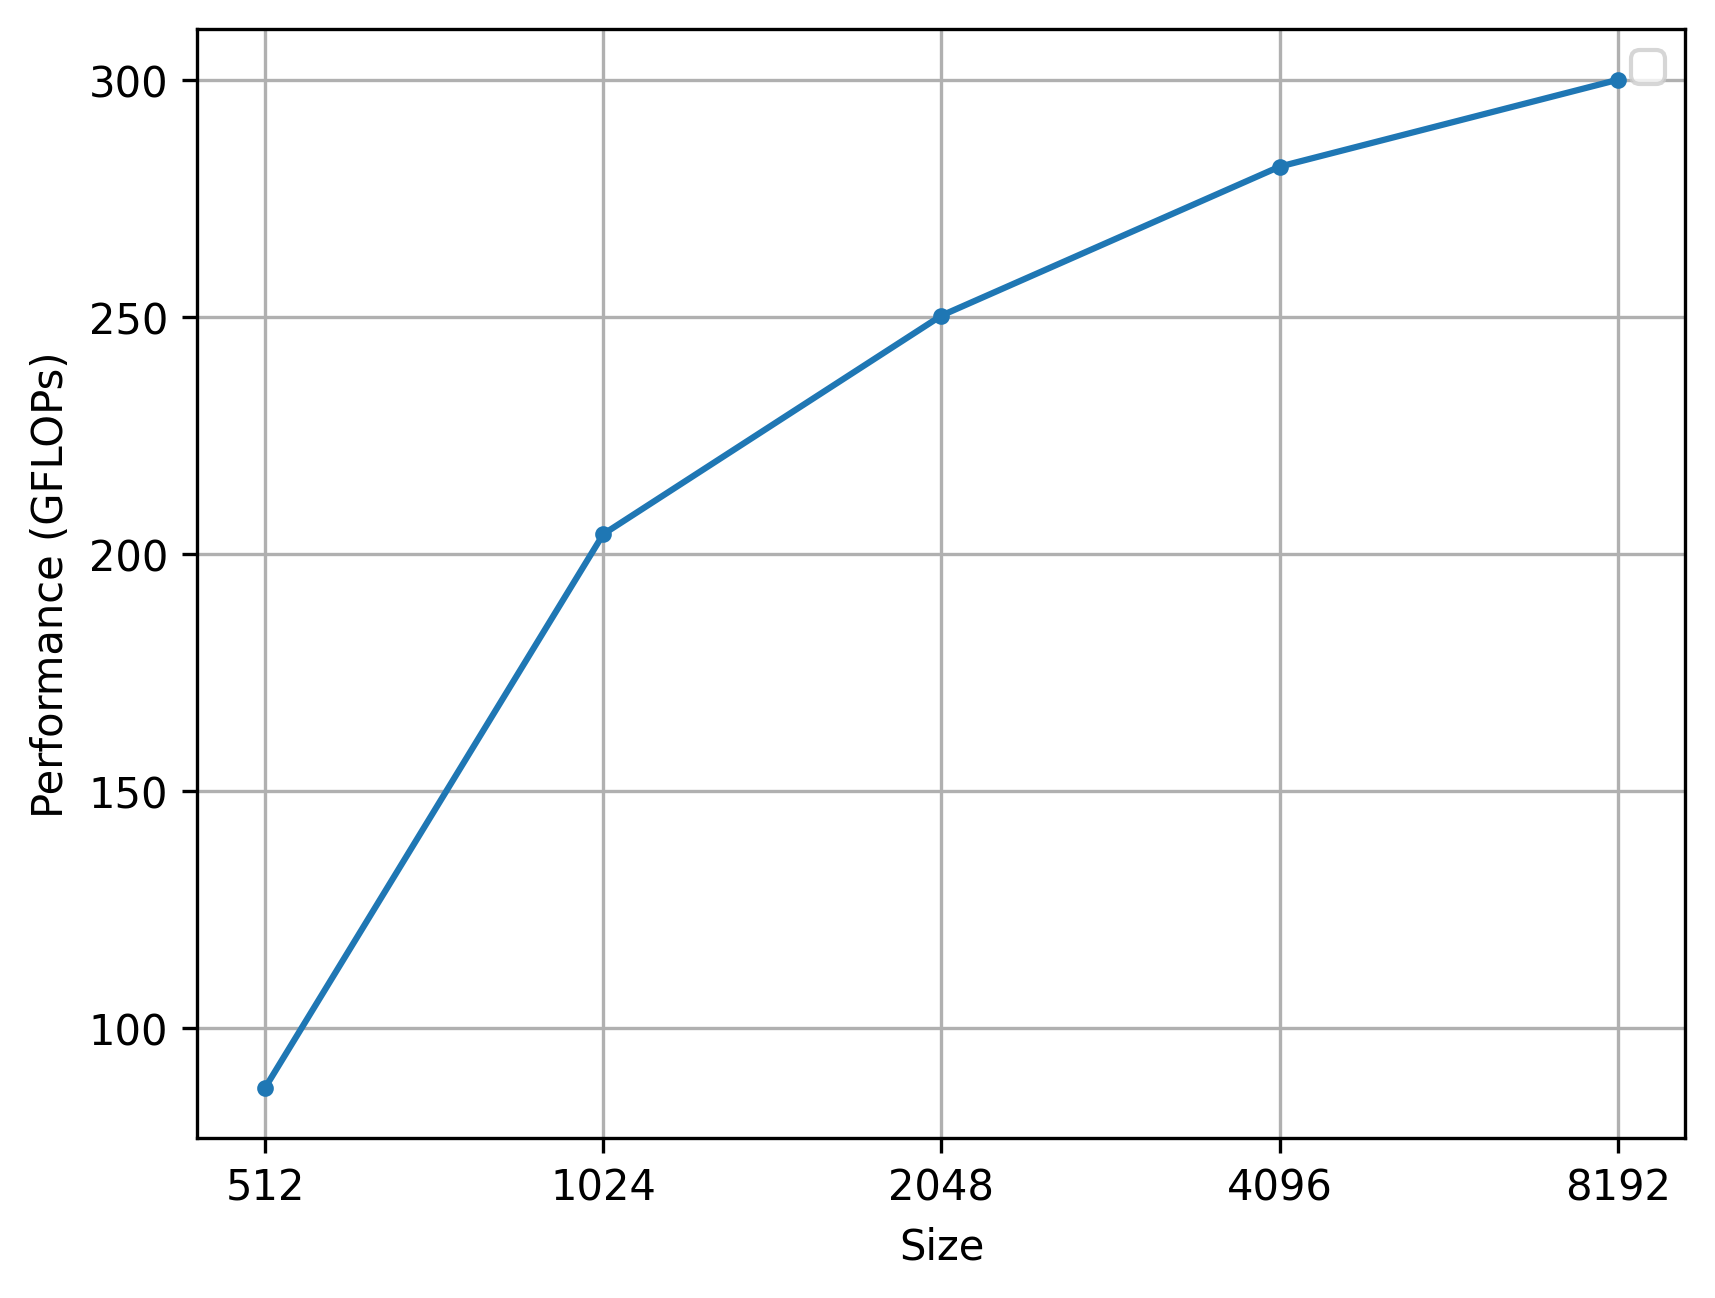
\includegraphics[width=\textwidth,height=8cm,keepaspectratio=true]{../figs/4.28Threads.png}
    \caption{Performance of DGEMM with 28 Threads, Different sizes}
    \label{fig:dgemm3}
\end{figure}

In our test, the performace got maximum at 300 GFLOPs when $S = 8192$, the trend line is still increase, but due to the limit in time, we could not test further on this.

\subsection{Bonus Task - DGEMM with Task-based}
Our full Task-based did not scale very well, we decided to present the performance hybrid version insteads. For that, insteads of a nested \textit{omp parallel for} loop OR a nested \textit{omp taskloop}, we combined both approaches - the outer loop is with \text{omp parallel for}, the inner loop is with \textit{omp taskloop}. We did some simple test to found out that the best performance is when the \textit{omp parallel for} loop has $nTeams$ while the contrain for $taskloop$ is with $grainsize(S/(N*threadsPerTeam*4))$, and $nThreadsPerTeam=2$. The comparison of this hybrid approach and our previous implementation is presented below: 

\begin{figure}[htpb]
    \centering
    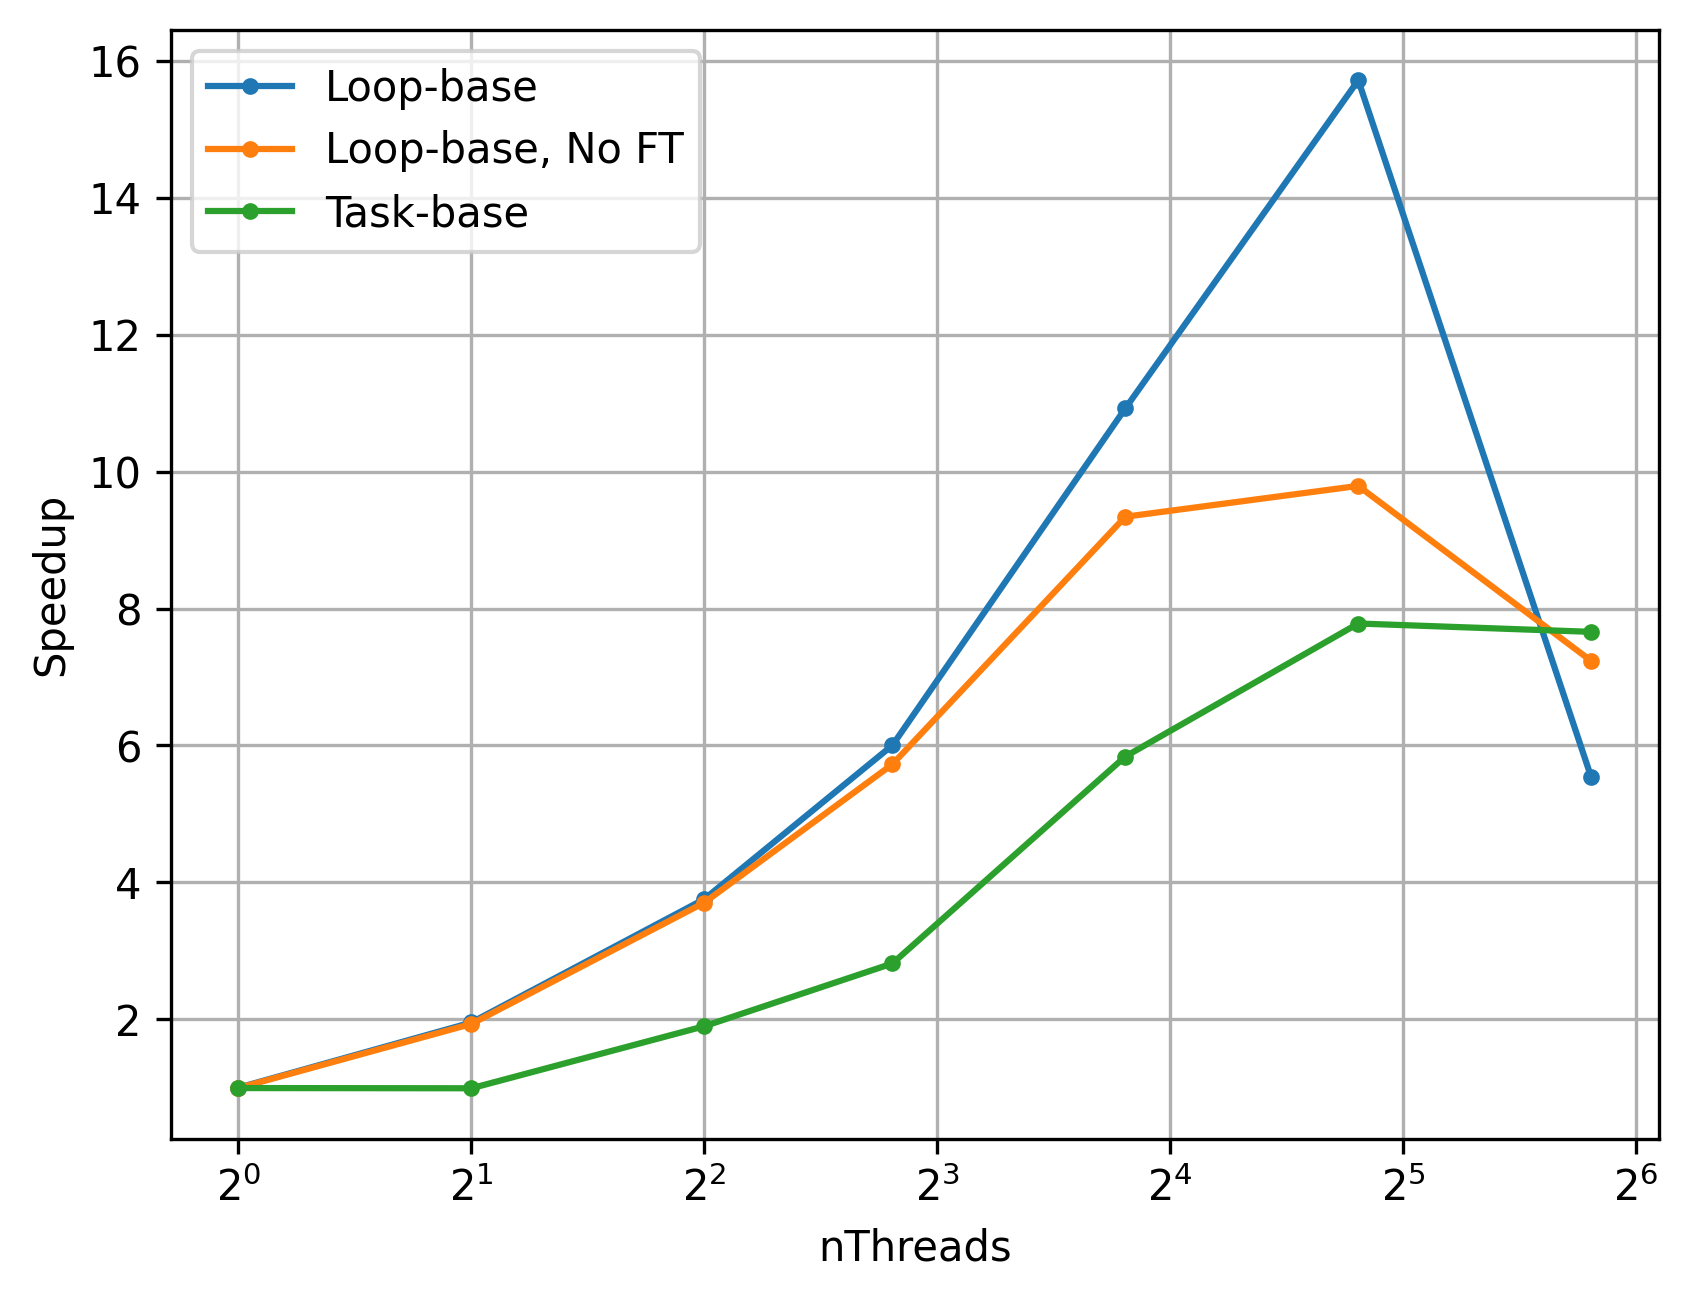
\includegraphics[width=\textwidth,height=8cm,keepaspectratio=true]{../figs/4.CompareTask.png}
    \caption{S=2048, Speedup of the Loop-based with and without First-touch, in comparison with Task-based}
    \label{fig:dgemm3}
\end{figure}
\textit{The speed up is normalized to the performance of Loop-based with First-touch with single thread} \\

This approach has performance scales in respect to number of threads, but does not have performance as good as the Loop-based one. Further constrains and optimisations are needed to get better performance.

\subsection{Conclusion}
Our best DGEMM performance is with S=8192, M=32, N=2, K=64, MC=32. With 28 threads, 2 threads/team, the performance is 300 GFLOPs.  
\medskip
%\printbibliography
\bibliography{myref}{}
\bibliographystyle{plain}

\end{document}


